% This must be in the first 5 lines to tell arXiv to use pdfLaTeX, which is strongly recommended.
\pdfoutput=1
% In particular, the hyperref package requires pdfLaTeX in order to break URLs across lines.

\documentclass[11pt]{article}

% Remove the "review" option to generate the final version.
%\usepackage[review]{acl}
\usepackage{acl}

% Standard package includes
\usepackage{times}
\usepackage{latexsym}

% For proper rendering and hyphenation of words containing Latin characters (including in bib files)
\usepackage[T1]{fontenc}
% For Vietnamese characters
% \usepackage[T5]{fontenc}
% See https://www.latex-project.org/help/documentation/encguide.pdf for other character sets

% This assumes your files are encoded as UTF8
\usepackage[utf8]{inputenc}

% This is not strictly necessary, and may be commented out,
% but it will improve the layout of the manuscript,
% and will typically save some space.
\usepackage{microtype}

% If the title and author information does not fit in the area allocated, uncomment the following
%
%\setlength\titlebox{<dim>}
%
% and set <dim> to something 5cm or larger.

\title{InstructEval: Systematic Evaluation of Instruction Selection Methods}

% Author information can be set in various styles:
% For several authors from the same institution:
% \author{Author 1 \and ... \and Author n \\
%         Address line \\ ... \\ Address line}
% if the names do not fit well on one line use
%         Author 1 \\ {\bf Author 2} \\ ... \\ {\bf Author n} \\
% For authors from different institutions:
% \author{Author 1 \\ Address line \\  ... \\ Address line
%         \And  ... \And
%         Author n \\ Address line \\ ... \\ Address line}
% To start a seperate ``row'' of authors use \AND, as in
% \author{Author 1 \\ Address line \\  ... \\ Address line
%         \AND
%         Author 2 \\ Address line \\ ... \\ Address line \And
%         Author 3 \\ Address line \\ ... \\ Address line}

\author{Anirudh Ajith$^{*}$ \quad Chris Pan$^{*}$\quad Mengzhou Xia \quad Ameet Deshpande \quad Karthik Narasimhan \\
\textnormal{Department of Computer Science, Princeton University} \\
\texttt{\{anirudh.ajith, chrispan, mengzhou, asd, karthikn\}@princeton.edu}
}

%%%%% Packages %%%%%
\usepackage{amsmath,amsfonts}
\usepackage{booktabs,arydshln}
\usepackage{multirow}
\usepackage{ulem}
\usepackage{pifont}
\usepackage{relsize}
\usepackage{enumitem}
\usepackage{graphicx}
\usepackage{amssymb}% http://ctan.org/pkg/amssymb
\usepackage{pifont}% http://ctan.org/pkg/pifont
\usepackage{dcolumn}
\usepackage{xcolor,colortbl}
\usepackage{supertabular}
\usepackage{tikz}
\usepackage{subcaption}
\usepackage{svg}
\usepackage{float}
\restylefloat{table}
\usepackage{enumitem}



%\usepackage[sfdefault,light]{FiraSans}
% \usepackage{minted}
% \usepackage[dvipsnames]{xcolor}

\newcolumntype{d}[1]{D{.}{.}{#1}}  % `d' column type aligns at decimal point

%%%%% Commands %%%%%
\newcommand{\cmark}{\ding{51}}%
\newcommand{\xmark}{\ding{55}}%
\newcommand{\greyrule}{\arrayrulecolor{black!30}\midrule\arrayrulecolor{black}}

%%%%%%%% Command for dashed lines %%%%%%%%
\makeatletter
\def\adl@drawiv#1#2#3{%
        \hskip.5\tabcolsep
        \xleaders#3{#2.5\@tempdimb #1{1}#2.5\@tempdimb}%
                #2\z@ plus1fil minus1fil\relax
        \hskip.5\tabcolsep}
\newcommand{\cdashlinelr}[1]{%
  \noalign{\vskip\aboverulesep
           \global\let\@dashdrawstore\adl@draw
           \global\let\adl@draw\adl@drawiv}
  \cdashline{#1}
  \noalign{\global\let\adl@draw\@dashdrawstore
           \vskip\belowrulesep}}
\makeatother


%%%%%%%% Review %%%%%%%%

\newcommand{\draftonly}[1]{#1} % uncomment to remove comments
\newcommand{\draftcomment}[3]{\draftonly{{\color{#2}{{{[#1: #3]}}}}}}
\newcommand{\anirudh}[1]{\draftcomment{Anirudh}{blue}{#1}}
\newcommand{\chris}[1]{\draftcomment{Chris}{teal}{#1}}
\newcommand{\ameet}[1]{\draftcomment{Ameet}{orange}{#1}}
\newcommand{\mz}[1]{\draftcomment{Mengzhou}{green}{#1}}
\newcommand{\karthik}[1]{\draftcomment{Karthik}{brown}{#1}}

%%%%%%%% Reference %%%%%%%%
\newcommand{\secref}[1]{Section~\ref{#1}}
\newcommand{\symbolsecref}[1]{($\S$~\ref{#1})}
\newcommand{\tableref}[1]{Table~\ref{#1}}
\newcommand{\figref}[1]{Figure~\ref{#1}}

\usetikzlibrary{backgrounds, shapes,arrows,positioning,matrix,fit}

\definecolor{lightblue}{RGB}{173,216,230}
\definecolor{lightpink}{RGB}{255,182,193}
\definecolor{lightyellow}{rgb}{0.9,0.9,0.6}
\definecolor{darkyellow}{rgb}{0.7, 0.7, 0.3}

\newcommand{\normalFont}[1]{\fontseries{m}\selectfont#1\fontseries{m}\selectfont}
\newcommand{\ultraLight}[1]{\fontseries{l}\selectfont#1\fontseries{m}\selectfont}

\pgfdeclarelayer{main}
\pgfdeclarelayer{layer1}
\pgfdeclarelayer{layer2}
\pgfdeclarelayer{layer3}
\pgfdeclarelayer{layer4}
\pgfdeclarelayer{layer5}
\pgfdeclarelayer{layer6}
\pgfsetlayers{layer6, layer5,layer4,layer3, layer2, layer1, main}


\begin{document}
\maketitle
\renewcommand{\thefootnote}{\fnsymbol{footnote}}
\footnotetext[1]{Equal contribution}
\renewcommand{\thefootnote}{\arabic{footnote}}

  In this paper, we explore the connection between secret key agreement and secure omniscience within the setting of the multiterminal source model with a wiretapper who has side information. While the secret key agreement problem considers the generation of a maximum-rate secret key through public discussion, the secure omniscience problem is concerned with communication protocols for omniscience that minimize the rate of information leakage to the wiretapper. The starting point of our work is a lower bound on the minimum leakage rate for omniscience, $\rl$, in terms of the wiretap secret key capacity, $\wskc$. Our interest is in identifying broad classes of sources for which this lower bound is met with equality, in which case we say that there is a duality between secure omniscience and secret key agreement. We show that this duality holds in the case of certain finite linear source (FLS) models, such as two-terminal FLS models and pairwise independent network models on trees with a linear wiretapper. Duality also holds for any FLS model in which $\wskc$ is achieved by a perfect linear secret key agreement scheme. We conjecture that the duality in fact holds unconditionally for any FLS model. On the negative side, we give an example of a (non-FLS) source model for which duality does not hold if we limit ourselves to communication-for-omniscience protocols with at most two (interactive) communications.  We also address the secure function computation problem and explore the connection between the minimum leakage rate for computing a function and the wiretap secret key capacity.
  
%   Finally, we demonstrate the usefulness of our lower bound on $\rl$ by using it to derive equivalent conditions for the positivity of $\wskc$ in the multiterminal model. This extends a recent result of Gohari, G\"{u}nl\"{u} and Kramer (2020) obtained for the two-user setting.
  
   
%   In this paper, we study the problem of secret key generation through an omniscience achieving communication that minimizes the 
%   leakage rate to a wiretapper who has side information in the setting of multiterminal source model.  We explore this problem by deriving a lower bound on the wiretap secret key capacity $\wskc$ in terms of the minimum leakage rate for omniscience, $\rl$. 
%   %The former quantity is defined to be the maximum secret key rate achievable, and the latter one is defined as the minimum possible leakage rate about the source through an omniscience scheme to a wiretapper. 
%   The main focus of our work is the characterization of the sources for which the lower bound holds with equality \textemdash it is referred to as a duality between secure omniscience and wiretap secret key agreement. For general source models, we show that duality need not hold if we limit to the communication protocols with at most two (interactive) communications. In the case when there is no restriction on the number of communications, whether the duality holds or not is still unknown. However, we resolve this question affirmatively for two-user finite linear sources (FLS) and pairwise independent networks (PIN) defined on trees, a subclass of FLS. Moreover, for these sources, we give a single-letter expression for $\wskc$. Furthermore, in the direction of proving the conjecture that duality holds for all FLS, we show that if $\wskc$ is achieved by a \emph{perfect} secret key agreement scheme for FLS then the duality must hold. All these results mount up the evidence in favor of the conjecture on FLS. Moreover, we demonstrate the usefulness of our lower bound on $\wskc$ in terms of $\rl$ by deriving some equivalent conditions on the positivity of secret key capacity for multiterminal source model. Our result indeed extends the work of Gohari, G\"{u}nl\"{u} and Kramer in two-user case.
% \leavevmode
% \\
% \\
% \\
% \\
% \\
\section{Introduction}
\label{introduction}

AutoML is the process by which machine learning models are built automatically for a new dataset. Given a dataset, AutoML systems perform a search over valid data transformations and learners, along with hyper-parameter optimization for each learner~\cite{VolcanoML}. Choosing the transformations and learners over which to search is our focus.
A significant number of systems mine from prior runs of pipelines over a set of datasets to choose transformers and learners that are effective with different types of datasets (e.g. \cite{NEURIPS2018_b59a51a3}, \cite{10.14778/3415478.3415542}, \cite{autosklearn}). Thus, they build a database by actually running different pipelines with a diverse set of datasets to estimate the accuracy of potential pipelines. Hence, they can be used to effectively reduce the search space. A new dataset, based on a set of features (meta-features) is then matched to this database to find the most plausible candidates for both learner selection and hyper-parameter tuning. This process of choosing starting points in the search space is called meta-learning for the cold start problem.  

Other meta-learning approaches include mining existing data science code and their associated datasets to learn from human expertise. The AL~\cite{al} system mined existing Kaggle notebooks using dynamic analysis, i.e., actually running the scripts, and showed that such a system has promise.  However, this meta-learning approach does not scale because it is onerous to execute a large number of pipeline scripts on datasets, preprocessing datasets is never trivial, and older scripts cease to run at all as software evolves. It is not surprising that AL therefore performed dynamic analysis on just nine datasets.

Our system, {\sysname}, provides a scalable meta-learning approach to leverage human expertise, using static analysis to mine pipelines from large repositories of scripts. Static analysis has the advantage of scaling to thousands or millions of scripts \cite{graph4code} easily, but lacks the performance data gathered by dynamic analysis. The {\sysname} meta-learning approach guides the learning process by a scalable dataset similarity search, based on dataset embeddings, to find the most similar datasets and the semantics of ML pipelines applied on them.  Many existing systems, such as Auto-Sklearn \cite{autosklearn} and AL \cite{al}, compute a set of meta-features for each dataset. We developed a deep neural network model to generate embeddings at the granularity of a dataset, e.g., a table or CSV file, to capture similarity at the level of an entire dataset rather than relying on a set of meta-features.
 
Because we use static analysis to capture the semantics of the meta-learning process, we have no mechanism to choose the \textbf{best} pipeline from many seen pipelines, unlike the dynamic execution case where one can rely on runtime to choose the best performing pipeline.  Observing that pipelines are basically workflow graphs, we use graph generator neural models to succinctly capture the statically-observed pipelines for a single dataset. In {\sysname}, we formulate learner selection as a graph generation problem to predict optimized pipelines based on pipelines seen in actual notebooks.

%. This formulation enables {\sysname} for effective pruning of the AutoML search space to predict optimized pipelines based on pipelines seen in actual notebooks.}
%We note that increasingly, state-of-the-art performance in AutoML systems is being generated by more complex pipelines such as Directed Acyclic Graphs (DAGs) \cite{piper} rather than the linear pipelines used in earlier systems.  
 
{\sysname} does learner and transformation selection, and hence is a component of an AutoML systems. To evaluate this component, we integrated it into two existing AutoML systems, FLAML \cite{flaml} and Auto-Sklearn \cite{autosklearn}.  
% We evaluate each system with and without {\sysname}.  
We chose FLAML because it does not yet have any meta-learning component for the cold start problem and instead allows user selection of learners and transformers. The authors of FLAML explicitly pointed to the fact that FLAML might benefit from a meta-learning component and pointed to it as a possibility for future work. For FLAML, if mining historical pipelines provides an advantage, we should improve its performance. We also picked Auto-Sklearn as it does have a learner selection component based on meta-features, as described earlier~\cite{autosklearn2}. For Auto-Sklearn, we should at least match performance if our static mining of pipelines can match their extensive database. For context, we also compared {\sysname} with the recent VolcanoML~\cite{VolcanoML}, which provides an efficient decomposition and execution strategy for the AutoML search space. In contrast, {\sysname} prunes the search space using our meta-learning model to perform hyperparameter optimization only for the most promising candidates. 

The contributions of this paper are the following:
\begin{itemize}
    \item Section ~\ref{sec:mining} defines a scalable meta-learning approach based on representation learning of mined ML pipeline semantics and datasets for over 100 datasets and ~11K Python scripts.  
    \newline
    \item Sections~\ref{sec:kgpipGen} formulates AutoML pipeline generation as a graph generation problem. {\sysname} predicts efficiently an optimized ML pipeline for an unseen dataset based on our meta-learning model.  To the best of our knowledge, {\sysname} is the first approach to formulate  AutoML pipeline generation in such a way.
    \newline
    \item Section~\ref{sec:eval} presents a comprehensive evaluation using a large collection of 121 datasets from major AutoML benchmarks and Kaggle. Our experimental results show that {\sysname} outperforms all existing AutoML systems and achieves state-of-the-art results on the majority of these datasets. {\sysname} significantly improves the performance of both FLAML and Auto-Sklearn in classification and regression tasks. We also outperformed AL in 75 out of 77 datasets and VolcanoML in 75  out of 121 datasets, including 44 datasets used only by VolcanoML~\cite{VolcanoML}.  On average, {\sysname} achieves scores that are statistically better than the means of all other systems. 
\end{itemize}


%This approach does not need to apply cleaning or transformation methods to handle different variances among datasets. Moreover, we do not need to deal with complex analysis, such as dynamic code analysis. Thus, our approach proved to be scalable, as discussed in Sections~\ref{sec:mining}.
\section{Related Work}
%\mz{We lack a comparison to this paper: https://arxiv.org/abs/2305.14877}
%\anirudh{refine to be more on-topic?}
\iffalse
\paragraph{In-Context Learning} As language models have scaled, the ability to learn in-context, without any weight updates, has emerged. \cite{brown2020language}. While other families of large language models have emerged, in-context learning remains ubiquitous \cite{llama, bloom, gptneo, opt}. Although such as HELM \cite{helm} have arisen for systematic evaluation of \emph{models}, there is no systematic framework to our knowledge for evaluating \emph{prompting methods}, and validating prompt engineering heuristics. The test-suite we propose will ensure that progress in the field of prompt-engineering is structured and objectively evaluated. 

\paragraph{Prompt Engineering Methods} Researchers are interested in the automatic design of high performing instructions for downstream tasks. Some focus on simple heuristics, such as selecting instructions that have the lowest perplexity \cite{lowperplexityprompts}. Other methods try to use large language models to induce an instruction when provided with a few input-output pairs \cite{ape}. Researchers have also used RL objectives to create discrete token sequences that can serve as instructions \cite{rlprompt}. Since the datasets and models used in these works have very little intersection, it is impossible to compare these methods objectively and glean insights. In our work, we evaluate these three methods on a diverse set of tasks and models, and analyze their relative performance. Additionally, we recognize that there are many other interesting angles of prompting that are not covered by instruction engineering \cite{weichain, react, selfconsistency}, but we leave these to future work.

\paragraph{Analysis of Prompting Methods} While most prompt engineering methods focus on accuracy, there are many other interesting dimensions of performance as well. For instance, researchers have found that for most tasks, the selection of demonstrations plays a large role in few-shot accuracy \cite{whatmakesgoodicexamples, selectionmachinetranslation, knnprompting}. Additionally, many researchers have found that even permuting the ordering of a fixed set of demonstrations has a significant effect on downstream accuracy \cite{fantasticallyorderedprompts}. Prompts that are sensitive to the permutation of demonstrations have been shown to also have lower accuracies \cite{relationsensitivityaccuracy}. Especially in low-resource domains, which includes the large public usage of in-context learning, these large swings in accuracy make prompting less dependable. In our test-suite we include sensitivity metrics that go beyond accuracy and allow us to find methods that are not only performant but reliable.

\paragraph{Existing Benchmarks} We recognize that other holistic in-context learning benchmarks exist. BigBench is a large benchmark of 204 tasks that are beyond the capabilities of current LLMs. BigBench seeks to evaluate the few-shot abilities of state of the art large language models, focusing on performance metrics such as accuracy \cite{bigbench}. Similarly, HELM is another benchmark for language model in-context learning ability. Rather than only focusing on performance, HELM branches out and considers many other metrics such as robustness and bias \cite{helm}. Both BigBench and HELM focus on ranking different language model, while fix a generic instruction and prompt format. We instead choose to evaluate instruction induction / selection methods over a fixed set of models. We are the first ever evaluation script that compares different prompt-engineering methods head to head. 
\fi

\paragraph{In-Context Learning and Existing Benchmarks} As language models have scaled, in-context learning has emerged as a popular paradigm and remains ubiquitous among several autoregressive LLM families \cite{brown2020language, llama, bloom, gptneo, opt}. Benchmarks like BigBench \cite{bigbench} and HELM \cite{helm} have been created for the holistic evaluation of these models. BigBench focuses on few-shot abilities of state-of-the-art large language models, while HELM extends to consider metrics like robustness and bias. However, these benchmarks focus on evaluating and ranking \emph{language models}, and do not address the systematic evaluation of \emph{prompting methods}. Although contemporary work by \citet{yang2023improving} also aims to perform a similar systematic analysis of prompting methods, they focus on simple probability-based prompt selection while we evaluate a broader range of methods including trivial instruction baselines, curated manually selected instructions, and sophisticated automated instruction selection.

\paragraph{Automated Prompt Engineering Methods} There has been interest in performing automated prompt-engineering for target downstream tasks within ICL. This has led to the exploration of various prompting methods, ranging from simple heuristics such as selecting instructions with the lowest perplexity \cite{lowperplexityprompts}, inducing instructions from large language models using a few annotated input-output pairs \cite{ape}, to utilizing RL objectives to create discrete token sequences as prompts \cite{rlprompt}. However, these works restrict their evaluation to small sets of models and tasks with little intersection, hindering their objective comparison. %\mz{For paragraphs that only have one work in the last line, try to shorten the paragraph to squeeze in context.}

\paragraph{Understanding in-context learning} There has been much recent work attempting to understand the mechanisms that drive in-context learning. Studies have found that the selection of demonstrations included in prompts significantly impacts few-shot accuracy across most tasks \cite{whatmakesgoodicexamples, selectionmachinetranslation, knnprompting}. Works like \cite{fantasticallyorderedprompts} also show that altering the ordering of a fixed set of demonstrations can affect downstream accuracy. Prompts sensitive to demonstration permutation often exhibit lower accuracies \cite{relationsensitivityaccuracy}, making them less reliable, particularly in low-resource domains.

Our work aims to bridge these gaps by systematically evaluating the efficacy of popular instruction selection approaches over a diverse set of tasks and models, facilitating objective comparison. We evaluate these methods not only on accuracy metrics, but also on sensitivity metrics to glean additional insights. We recognize that other facets of prompting not covered by instruction engineering exist \cite{weichain, react, selfconsistency}, and defer these explorations to future work. 
\section{Evaluation Suite}
%We design a comprehensive evaluation suite to assess the performance of instructions along 5 metrics relevant to practical ICL. To ensure a fair analysis, we test each instruction selection method across 9 tasks and 13 autoregressive models from 4 model families.

\subsection{Prompt format}

\begin{figure}[t]
    \centering
    %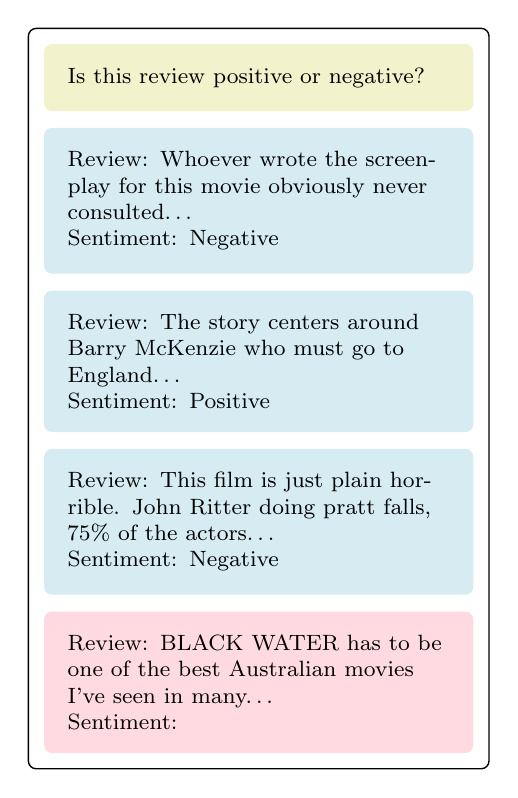
\begin{tikzpicture}[
  node distance = 0.2cm and 0.2cm,
  single node/.style = {rectangle, fill=#1, fill opacity=0.5, text opacity=1, align=left, font=\fontfamily{FiraSans-LF}\selectfont\footnotesize, text width=0.40\textwidth, inner xsep=3mm, inner ysep=3mm, rounded corners=1mm},
]

\node[single node=lightyellow] (instruction) 
{\normalFont{Is this review positive or negative?}};

\node[single node=lightblue, below=of instruction] (example1)
{\normalFont{Review:} \ultraLight{Whoever wrote the screenplay for this movie obviously never consulted…} \\ \normalFont{Sentiment:} \ultraLight{Negative}};

\node[single node=lightblue, below=of example1] (example2)
{\normalFont{Review:} \ultraLight{The story centers around Barry McKenzie who must go to England…} \\ \normalFont{Sentiment:} \ultraLight{Positive}};

\node[single node=lightblue, below=of example2] (example3)
{\normalFont{Review:} \ultraLight{This film is just plain horrible. John Ritter doing pratt falls, 75\% of the actors…} \\ \normalFont{Sentiment:} \ultraLight{Negative}};


\node[single node=lightpink, below=of example3] (test) 
{\normalFont{Review:} \ultraLight{BLACK WATER has to be one of the best Australian movies I've seen in many…} \\ \normalFont{Sentiment:} };

\draw [black, line width=0.5pt, rounded corners=1mm] ([shift={(-2mm,-2mm)}]current bounding box.south west) rectangle ([shift={(2mm,2mm)}]current bounding box.north east);

\end{tikzpicture}
    \includegraphics[width=\linewidth]{figures/prompt_example.png}
    \caption{
        An example of a prompt following the template we use for IMDB. By  `prompt' we refer to the concatenation of the \textcolor{darkyellow}{instruction}, solved \textcolor{blue}{demonstrations} and an unsolved \textcolor{red}{test example}.
    }
    \label{fig:prompt_example}
\end{figure}
We define a `prompt' as the full textual input provided to an LLM. Our evaluation suite supports the use of any number of demonstrations, arbitrary demonstration templates and the inclusion of custom strings anywhere within the prompt. Since the instructions used can be set to any arbitrary strings, users are free to use any external means to select instructions and have them evaluated by our suite.

For consistency, we conduct all experiments in this work using prompts that begin with an instruction, continue with a sequence of annotated training demonstrations, and conclude with an unsolved test example\footnote{Instructions are omitted during `Null instruction' evaluations. Demonstrations are omitted in zero-shot evaluations.} (Figure~\ref{fig:prompt_example}), and express each example in a minimal, task-specific key-value format (Table~\ref{table:templates}) that reflects task semantics.

\subsection{Metrics}
\begin{figure*}
  \begin{subfigure}[b]{0.32\textwidth}
    \centering
    \resizebox{\linewidth}{!}{
    \iffalse

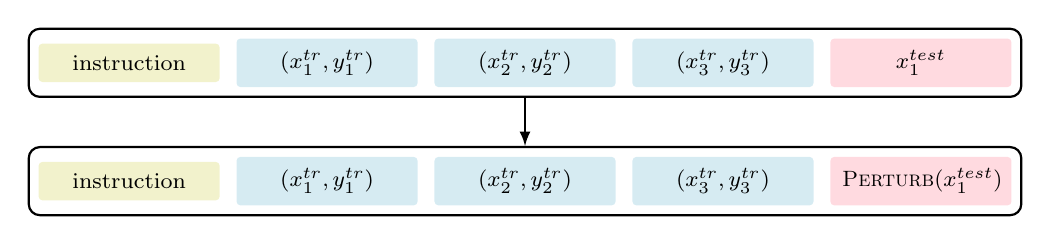
\begin{tikzpicture}[
  node distance = 0.2cm and 0.2cm,
  single node/.style = {rectangle, fill=#1, text opacity=1, opacity=0.5, align=center, font=\footnotesize, text width=2cm, inner sep=1.5mm, rounded corners=0.5mm},
  bigbox/.style = {draw, thick, rounded corners, rectangle},
  arrow/.style={thick, -latex},
]

\node[single node=lightyellow] (instruction) {instruction};

\node[single node=lightblue, right=of instruction] (example1) {$(x_1^{tr}, y_1^{tr})$};
\node[single node=lightblue, right=of example1] (example2) {$(x_2^{tr}, y_2^{tr})$};
\node[single node=lightblue, right=of example2] (example3) {$(x_3^{tr}, y_3^{tr})$};

\node[single node=lightpink, right=of example3] (test) {$x_1^{test}$};

\node[bigbox, fit=(instruction) (example1) (example2) (example3) (test)] (box1) {};

\node[single node=lightyellow, below=1cm of instruction] (instruction2) {instruction};

\node[single node=lightblue, right=of instruction2] (example12) {$(x_1^{tr}, y_1^{tr})$};
\node[single node=lightblue, right=of example12] (example22) {$(x_2^{tr}, y_2^{tr})$};
\node[single node=lightblue, right=of example22] (example32) {$(x_3^{tr}, y_3^{tr})$};

\node[single node=lightpink, right=of example32] (test2) {\textsc{Perturb}$(x_1^{test})$};

\node[bigbox, fit=(instruction2) (example12) (example22) (example32) (test2)] (box2) {};

\draw [arrow] (box1.south) -- (box2.north);

\end{tikzpicture}

\fi


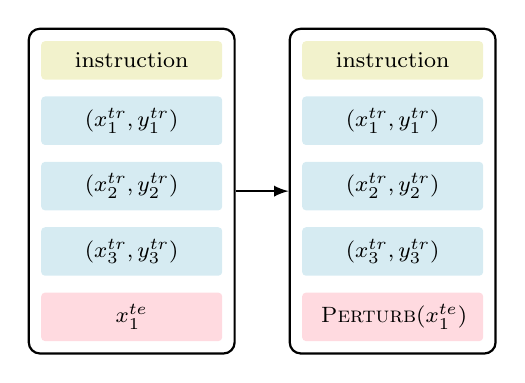
\begin{tikzpicture}[
  node distance = 0.2cm and 1cm, % Increase horizontal distance between nodes
  single node/.style = {rectangle, fill=#1, text opacity=1, opacity=0.5, align=center, font=\footnotesize, text width=2cm, inner sep=1.5mm, rounded corners=0.5mm},
  bigbox/.style = {draw, thick, rounded corners, rectangle, inner sep=1.5mm}, % Reduce inner sep for less padding
  arrow/.style={thick, -latex},
]

\node[single node=lightyellow] (instruction1) {instruction};
\node[single node=lightblue, below=of instruction1] (example1) {$(x_1^{tr}, y_1^{tr})$};
\node[single node=lightblue, below=of example1] (example2) {$(x_2^{tr}, y_2^{tr})$};
\node[single node=lightblue, below=of example2] (example3) {$(x_3^{tr}, y_3^{tr})$};
\node[single node=lightpink, below=of example3] (test1) {$x_1^{te}$};

\node[bigbox, fit=(instruction1) (example1) (example2) (example3) (test1)] (box1) {};

\node[single node=lightyellow, right=of instruction1] (instruction2) {instruction};
\node[single node=lightblue, below=of instruction2] (example12) {$(x_1^{tr}, y_1^{tr})$};
\node[single node=lightblue, below=of example12] (example22) {$(x_2^{tr}, y_2^{tr})$};
\node[single node=lightblue, below=of example22] (example32) {$(x_3^{tr}, y_3^{tr})$};
\node[single node=lightpink, below=of example32] (test2) {\textsc{Perturb}$(x_1^{te})$};

\node[bigbox, fit=(instruction2) (example12) (example22) (example32) (test2)] (box2) {};

\draw [arrow] (box1.east) -- (box2.west);
\end{tikzpicture}

    }
    \caption{Perturbation accuracy}
  \end{subfigure}\hfill
  \begin{subfigure}[b]{0.32\textwidth}
    \centering
    \resizebox{\linewidth}{!}{
    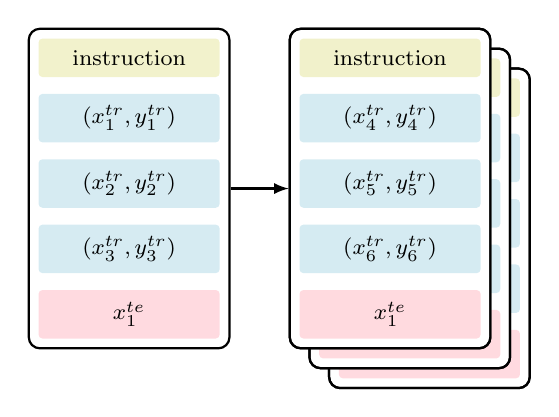
\begin{tikzpicture}[
  node distance = 0.2cm and 0.2cm,
  single node/.style = {rectangle, fill=#1, text opacity=1, opacity=0.5, align=center, font=\footnotesize, text width=2cm, inner sep=1.5mm, rounded corners=0.5mm},
  bigbox/.style = {draw, thick, rounded corners, rectangle},
  arrow/.style={thick, -latex},
  bigbox opaque/.style = {draw, thick, rounded corners, rectangle, opacity=1, fill=white},
  arrow/.style={thick, -latex},
]

\node[single node=lightyellow] (instruction) {instruction};

\node[single node=lightblue, below=of instruction] (example1) {$(x_1^{tr}, y_1^{tr})$};
\node[single node=lightblue, below=of example1] (example2) {$(x_2^{tr}, y_2^{tr})$};
\node[single node=lightblue, below=of example2] (example3) {$(x_3^{tr}, y_3^{tr})$};

\node[single node=lightpink, below=of example3] (test) {$x_1^{te}$};

\node[bigbox, fit=(instruction) (example1) (example2) (example3) (test)] (box1) {};

\begin{pgfonlayer}{layer1}
\node[single node=lightyellow, right=1cm of instruction] (instruction2) {instruction};

\node[single node=lightblue, below=of instruction2] (example12) {$(x_4^{tr}, y_4^{tr})$};
\node[single node=lightblue, below=of example12] (example22) {$(x_5^{tr}, y_5^{tr})$};
\node[single node=lightblue, below=of example22] (example32) {$(x_6^{tr}, y_6^{tr})$};

\node[single node=lightpink, below=of example32] (test2) {$x_1^{te}$};

\node[bigbox, fit=(instruction2) (example12) (example22) (example32) (test2)] (box2) {};
\end{pgfonlayer}

\begin{pgfonlayer}{layer2}
\node[bigbox opaque, fit=(instruction2) (example12) (example22) (example32) (test2)] (box2) {};
\end{pgfonlayer}

\begin{pgfonlayer}{layer3}
\node[single node=lightyellow, below=-0.25cm of instruction2, xshift=0.25cm] (instruction3) {instruction};

\node[single node=lightblue, below=of instruction3] (example13) {$(x_1^{tr}, y_1^{tr})$};
\node[single node=lightblue, below=of example13] (example23) {$(x_2^{tr}, y_2^{tr})$};
\node[single node=lightblue, below=of example23] (example33) {$(x_3^{tr}, y_3^{tr})$};

\node[single node=lightpink, below=of example33] (test3) {$x_1^{test}$};

\node[bigbox, fit=(instruction3) (example13) (example23) (example33) (test3)] (box3) {};
\end{pgfonlayer}

\begin{pgfonlayer}{layer4}
\node[bigbox opaque, fit=(instruction3) (example13) (example23) (example33) (test3)] (box3) {};
\end{pgfonlayer}

\begin{pgfonlayer}{layer5}
\node[single node=lightyellow, below=-0.25cm of instruction3, xshift=0.25cm] (instruction4) {instruction};

\node[single node=lightblue, below=of instruction4] (example14) {$(x_1^{tr}, y_1^{tr})$};
\node[single node=lightblue, below=of example14] (example24) {$(x_2^{tr}, y_2^{tr})$};
\node[single node=lightblue, below=of example24] (example34) {$(x_3^{tr}, y_3^{tr})$};

\node[single node=lightpink, below=of example34] (test4) {$x_1^{test}$};

\node[bigbox, fit=(instruction4) (example14) (example24) (example34) (test4)] (box4) {};
\end{pgfonlayer}

\begin{pgfonlayer}{layer6}
\node[bigbox, fit=(instruction4) (example14) (example24) (example34) (test4)] (box4) {};
\end{pgfonlayer}

\draw [arrow] (box1.east) -- (box2.west);

\end{tikzpicture}

    }
    \caption{Selectional sensitivity}
  \end{subfigure}\hfill
  \begin{subfigure}[b]{0.32\textwidth}
    \centering
    \resizebox{\linewidth}{!}{
    \iffalse
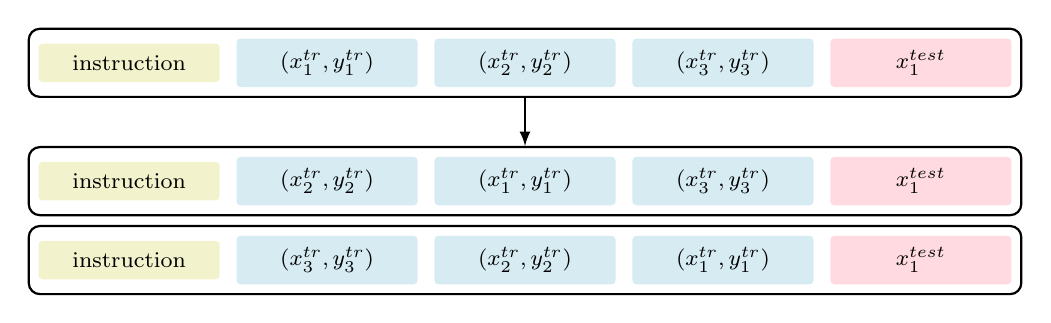
\begin{tikzpicture}[
  node distance = 0.2cm and 0.2cm,
  single node/.style = {rectangle, fill=#1, text opacity=1, opacity=0.5, align=center, font=\footnotesize, text width=2cm, inner sep=1.5mm, rounded corners=0.5mm},
  bigbox/.style = {draw, thick, rounded corners, rectangle},
  arrow/.style={thick, -latex},
]

\node[single node=lightyellow] (instruction) {instruction};

\node[single node=lightblue, right=of instruction] (example1) {$(x_1^{tr}, y_1^{tr})$};
\node[single node=lightblue, right=of example1] (example2) {$(x_2^{tr}, y_2^{tr})$};
\node[single node=lightblue, right=of example2] (example3) {$(x_3^{tr}, y_3^{tr})$};

\node[single node=lightpink, right=of example3] (test) {$x_1^{test}$};

\node[bigbox, fit=(instruction) (example1) (example2) (example3) (test)] (box1) {};

\node[single node=lightyellow, below=1cm of instruction] (instruction2) {instruction};

\node[single node=lightblue, right=of instruction2] (example12) {$(x_2^{tr}, y_2^{tr})$};
\node[single node=lightblue, right=of example12] (example22) {$(x_1^{tr}, y_1^{tr})$};
\node[single node=lightblue, right=of example22] (example32) {$(x_3^{tr}, y_3^{tr})$};

\node[single node=lightpink, right=of example32] (test2) {$x_1^{test}$};

\node[bigbox, fit=(instruction2) (example12) (example22) (example32) (test2)] (box2) {};

\draw [arrow] (box1.south) -- (box2.north);

\node[single node=lightyellow, below=0.5cm of instruction2] (instruction3) {instruction};

\node[single node=lightblue, right=of instruction3] (example13) {$(x_3^{tr}, y_3^{tr})$};
\node[single node=lightblue, right=of example13] (example23) {$(x_2^{tr}, y_2^{tr})$};
\node[single node=lightblue, right=of example23] (example33) {$(x_1^{tr}, y_1^{tr})$};

\node[single node=lightpink, right=of example33] (test3) {$x_1^{test}$};

\node[bigbox, fit=(instruction3) (example13) (example23) (example33) (test3)] (box3) {};


\end{tikzpicture}
\fi



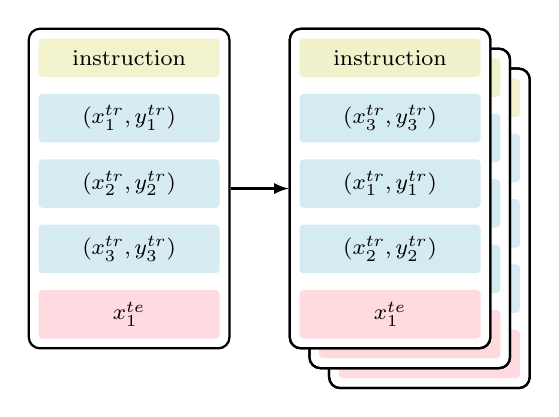
\begin{tikzpicture}[
  node distance = 0.2cm and 0.2cm,
  single node/.style = {rectangle, fill=#1, text opacity=1, opacity=0.5, align=center, font=\footnotesize, text width=2cm, inner sep=1.5mm, rounded corners=0.5mm},
  bigbox/.style = {draw, thick, rounded corners, rectangle},
  arrow/.style={thick, -latex},
  bigbox opaque/.style = {draw, thick, rounded corners, rectangle, opacity=1, fill=white},
  arrow/.style={thick, -latex},
]

\node[single node=lightyellow] (instruction) {instruction};

\node[single node=lightblue, below=of instruction] (example1) {$(x_1^{tr}, y_1^{tr})$};
\node[single node=lightblue, below=of example1] (example2) {$(x_2^{tr}, y_2^{tr})$};
\node[single node=lightblue, below=of example2] (example3) {$(x_3^{tr}, y_3^{tr})$};

\node[single node=lightpink, below=of example3] (test) {$x_1^{te}$};

\node[bigbox, fit=(instruction) (example1) (example2) (example3) (test)] (box1) {};

\begin{pgfonlayer}{layer1}
\node[single node=lightyellow, right=1cm of instruction] (instruction2) {instruction};

\node[single node=lightblue, below=of instruction2] (example12) {$(x_3^{tr}, y_3^{tr})$};
\node[single node=lightblue, below=of example12] (example22) {$(x_1^{tr}, y_1^{tr})$};
\node[single node=lightblue, below=of example22] (example32) {$(x_2^{tr}, y_2^{tr})$};

\node[single node=lightpink, below=of example32] (test2) {$x_1^{te}$};

\node[bigbox, fit=(instruction2) (example12) (example22) (example32) (test2)] (box2) {};
\end{pgfonlayer}

\begin{pgfonlayer}{layer2}
\node[bigbox opaque, fit=(instruction2) (example12) (example22) (example32) (test2)] (box2) {};
\end{pgfonlayer}

\begin{pgfonlayer}{layer3}
\node[single node=lightyellow, below=-0.25cm of instruction2, xshift=0.25cm] (instruction3) {instruction};

\node[single node=lightblue, below=of instruction3] (example13) {$(x_1^{tr}, y_1^{tr})$};
\node[single node=lightblue, below=of example13] (example23) {$(x_2^{tr}, y_2^{tr})$};
\node[single node=lightblue, below=of example23] (example33) {$(x_3^{tr}, y_3^{tr})$};

\node[single node=lightpink, below=of example33] (test3) {$x_1^{test}$};

\node[bigbox, fit=(instruction3) (example13) (example23) (example33) (test3)] (box3) {};
\end{pgfonlayer}

\begin{pgfonlayer}{layer4}
\node[bigbox opaque, fit=(instruction3) (example13) (example23) (example33) (test3)] (box3) {};
\end{pgfonlayer}

\begin{pgfonlayer}{layer5}
\node[single node=lightyellow, below=-0.25cm of instruction3, xshift=0.25cm] (instruction4) {instruction};

\node[single node=lightblue, below=of instruction4] (example14) {$(x_1^{tr}, y_1^{tr})$};
\node[single node=lightblue, below=of example14] (example24) {$(x_2^{tr}, y_2^{tr})$};
\node[single node=lightblue, below=of example24] (example34) {$(x_3^{tr}, y_3^{tr})$};

\node[single node=lightpink, below=of example34] (test4) {$x_1^{test}$};

\node[bigbox, fit=(instruction4) (example14) (example24) (example34) (test4)] (box4) {};
\end{pgfonlayer}

\begin{pgfonlayer}{layer6}
\node[bigbox, fit=(instruction4) (example14) (example24) (example34) (test4)] (box4) {};
\end{pgfonlayer}

\draw [arrow] (box1.east) -- (box2.west);

\end{tikzpicture}
    }
    \caption{Permutational sensitivity}
  \end{subfigure}
  \caption{
        We provide schematic diagrams that show prompts are modified to measure \textit{perturbation accuracy}, \textit{selectional sensitivity} and \textit{permutational sensitivity}. We perturb the test input to measure perturbation accuracy, and demonstration selection and permutation respectively while measuring selectional and permutational sensitivity.
    }
    \label{fig:sensitivity-metrics}
\end{figure*}

\label{sec:metrics}
\paragraph{Accuracy metrics} Accuracy is typically the primary metric of interest in ICL. While ICL is most commonly performed in few-shot settings where a handful of annotated demonstrations are included in the prompt, models are also prompted zero-shot without the use of such demonstrations. Since real-world scenarios can often contain grammatical errors and misspellings in the test input, it is desirable to find prompts robust to these perturbations. Hence, we measure \textit{zero-shot accuracy}, \textit{few-shot accuracy}, and \textit{perturbation accuracy}\footnote{We choose to treat this as an accuracy metric rather than a sensitivity metric since it is not meaningful to measure sensitivity to such perturbations in situations where a prompt only elicits near random-chance task performance from a model.} in our evaluations. Following \citet{helm}, we measure perturbation accuracy by introducing random capitalization, spacing, contractions and common misspellings in the test input.

\paragraph{Sensitivity metrics} Previous work has shown that the accuracy obtained using a prompt template can fluctuate significantly as a function of the set of demonstrations included in the prompt ~\cite{Liu2021WhatMG, Su2022SelectiveAM, rubin2022learning, Wang2023LargeLM} and the order they are presented in \cite{fantasticallyorderedprompts}. It may be desirable in practice to identify prompt templates and instructions that offer consistent performance regardless of the choice of demonstrations and their arrangement. Hence, we introduce \textit{selectional sensitivity} and \textit{permutational sensitivity} metrics to measure the sensitivity of chosen instructions respectively to selected demonstrations, and the order in which they are arranged. We quantify the sensitivity of an instruction (given a model and task) using the standard deviation of accuracies obtained on varying  the selection or permutation of the demonstrations used, each across 16 random choices.

\subsection{Aggregating metrics across Models}

Each instruction selection method being tested across $N$ models and $M$ datasets yields $NM$ values per metric. Comparing these $NM$-dimensional vectors directly is complex. It can be challenging to reduce them to a single representative scalar. Simple approaches such as computing the mean of these $NM$ values can prove inadequate since the resulting scores would tend to be heavily influenced by metric values that exhibit a high variance across different inspected methods. 

We opt against using aggregation techniques used by previous works \cite{helm, bigbench} due to their drawbacks (Section~\ref{app:scoring}) and instead adopt `mean relative gain' as a means to aggregate accuracy metrics across multiple models. We rely on simple averaging for sensitivity metrics, partly because we observe that these quantities do not show much variation across methods.

\subsubsection{Accuracy metrics}
Considering the range of models and datasets in our evaluation suite, we unsurprisingly observe substantial variation in accuracy magnitudes across model scales and tasks. However, we notice that the degree of variation in accuracy due to instruction choice is usually considerably smaller than the degree of variation due to model and task choice.

To meaningfully compare and aggregate the relative performance of different instruction selection methods across models, we use a measure called \textit{mean relative gain}. First, we define the \textit{relative gain} for a value $x$ from a population $P$ as the percentage by which $x$ exceeds the mean value of $P$:

$$\text{r-gain}_P(x) = 100 \times \dfrac{x-\mu_P}{\mu_P}$$

Consider a collection of models $\mathcal{M}$ and instructions $\mathcal{I}$ for a task $t$. Given a model $m$, we calculate the raw accuracy scores $s_{tmi}$ for each instruction $i \in \mathcal{I}$. Taking this set $S_{tm}$ to be the population, we compare the performances of the instructions against each other by computing their corresponding relative gains $r_{tmi} = \text{r-gain}_{S_{tm}}(s_{tmi})$. Each $r_{tmi}$ represents the degree by which method $i$ outperforms the average performance along the metric on task $t$ for model $m$.

We now define the mean relative gain as 
$$\overline{r}_{ti} = \dfrac{1}{|\mathcal{M}|} \sum_{m \in \mathcal{M}} r_{tmi}$$

These $\overline{r}_{ti}$ values, tabulated and analyzed in \secref{sec:results}, capture not only the ordinal information about each method's performance on a given task but also provide an intuitive sense of the magnitude by which these methods outperform others. Specifically, if an induction method $i$ has a mean relative gain $\overline{r}_{ti}$ on task $t$, this means that method $i$ exceeds average performance (across $\mathcal{I}$) on task $t$ by $\overline{r}_{ti}$ percent when averaged across models $\mathcal{M}$. 

\subsubsection{Sensitivity metrics}
To aggregate the sensitivity of an instruction selection/induction method $i$ over all models for a task $t$, we simply compute the average of the raw sensitivity scores (described in \secref{sec:metrics}). Specifically, if $\sigma_{tmi}$ is the raw sensitivity score obtained for model $m$ and task $t$ when using instruction $i$, then the aggregated sensitivity score $\overline{\sigma}_{ti}$ is given by 

$$\overline{\sigma}_{ti} = \dfrac{1}{|\mathcal{M}|} \sum_{m \in \mathcal{M}} \sigma_{tmi}$$

We choose to avoid more sophisticated aggregation strategies like relative gain for sensitivity metrics since standard deviations are already secondary metrics making it unintuitive to discuss the relative gain of the standard deviation obtained using a method over the average. %\mz{Do we still average the stds? It seems that in table 5 we didn't do it?}

\iffalse
To fairly compare instruction induction methods across various models and tasks, we adopt mean z-scores as a measure of relative performance along a specific metric. This choice allows us to capture the magnitude of variation in the underlying metric without requiring expert knowledge about its specific range of variation.~\footnote{Please refer to Appendix \ref{app:scoring} for more detailed information on why we opted not to use head-to-head win rates from HELM~\cite{helm} and normalized accuracy from BigBench~\cite{bigbench} as alternative scoring methods.}

A z-score measures the relationship between a value and the population it is drawn from. It quantifies how many standard deviations a value $x$ is away from the mean of the population $P$:
$$\text{z-score}_{P}(x) = \dfrac{x - \mu_P}{\sigma_P},$$
Let $s_{pmt}$ represent the raw scores of each instruction induction method $p$ for model $m$ and task $t$. We denote the subset of these metric scores associated with each pair $(m,t)$ as $$S(m,t) = \{s_{pmt}: p \in \mathcal{P}\}.$$ We compute the z-score for metric scores within each $S(m, t)$ and group them by a method $p$:
$$Z_p = \{\text{z-score}_{S(m,t)}(s_{pmt}) : (m,t) \in \mathcal{M} \times \mathcal{T}\}.$$
We then take an average and derive the mean z-score for $p$ across tasks and models:
$$\overline{z}_p = \sum_{z_p \in Z_p} z_p / |Z_p|$$

These mean z-score values are indicative of the degree to which each instruction induction method outperforms all other method under consideration along a certain metric, aggregated over all possible choices of models in $\mathcal{M}$ and tasks in $\mathcal{T}$.  Although they do communicate the magnitude by which certain methods outperform others, they are indeed bound by the limitation that they have to be recomputed for all $p$ whenever a new method $p'$ is inserted into $\mathcal{P}$. However, this limitation is shown by scoring systems used in previous works \cite{helm} as well and is not a cause for concern in practice when evaluating the relative performances of instruction induction methods.
\fi


\subsection{Tasks}
\begin{table}[t]
\centering
\resizebox{\linewidth}{!}{
\begin{tabular}{ll}
\toprule
\textbf{Task Type} & \textbf{Tasks} \\ 
\midrule
\multirow{5}{*}{Classification (CLS)}      & AG News \cite{agnews} \\ 
                                            & ANLI \cite{anli} \\
                                            & BoolQ \cite{boolq} \\ 
                                            & IMDB \cite{imdb} \\ 
                                            & TweetEval Emotion \cite{emotion} \\
\midrule                                            
\multirow{2}{*}{Multiple-choice (MCQ)}                      & CosmosQA \cite{cosmosqa} \\ 
& HellaSwag \cite{hellaswag} \\
\midrule
\multirow{2}{*}{Generative QA (GQA)}                         & NQ-Open \cite{nqopen} \\ 
& TriviaQA \cite{triviaqa} \\ \bottomrule
\end{tabular}}
\caption{Tasks included in our evaluation suite.}
\label{table:tasks}
\end{table} 
While previous instruction induction \cite{ape, rlprompt} work has tended to focus mostly on classification tasks, we include 9 tasks (\tableref{table:tasks}) in our evaluation suite spanning classification (CLS), multiple-choice question-answering (MCQ) and generative question-answering (GQA) to assess the applicability of instruction selection and induction methods to other task-types as well. We concentrate on tasks that are challenging to contemporary language models, and yet are not so demanding that the performance of these models does not exceed random chance. We exclude certain generative tasks, like summarization, which are challenging to assess objectively.~\footnote{Standard summarization metrics correlate poorly with human preferences~\cite{helm, goyal2023news}.}

\section{Model and Optimization}
\vspace{-2mm}
\label{sec:model}
\setlength{\textfloatsep}{\textfloatsepsave}
We use the {\em attentional neural \encdec} model \cite{2014arXiv1409.0473B} as a basis for both \proposed and \mle.
The model takes (possibly ungrammatical) source sentences $x \in X$ as an input, and predicts grammatical and fluent output sentences $y \in Y$ according to the model parameter $\theta$.
The model consists of two sub-modules, {\em encoder} and {\em decoder}. 
The encoder transforms $x$ into a sequence of vector representations (hidden states) using a bidirectional gated recurrent neural network (GRU) \cite{2014arXiv1412.3555C}.
The decoder predicts a word $y_t$ at a time, using previous token $y_{t-1}$ and linear combination of encoder information as attention.
%With the encoder representation, the decoder predicts a word $y_t$ with previous information at each time step.
%% MJP: I think you could just delete the rest of the subsection (the equation and next two sentences)
%\todo{definition of $\theta$}
%Thus, the entire \encdec model is formalized as follows:
%\begin{eqnarray}
%p(y|x;\theta) = \sum_{t=1}^{T}p(y_{t}|x, y_1^{t-1};\theta)
%\end{eqnarray}
%
%For more technical details such as attention mechanism, refer to \newcite{2014arXiv1409.0473B}.
%\todo{or should I describe it in the Appendix?}

%%%%%%%%%%%%%%%%%%%%%%%%%%%%%%%
\vspace{-1mm}
\subsection{Maximum Likelihood Estimation}
\vspace{-1mm}
\label{sec:mle}
Maximum Likelihood Estimation training (\mle) is a standard optimization method for \encdec models.
In \mle, the objective is to maximize the log likelihood of the correct sequence for a given sequence for the entire training data.
\begin{eqnarray}
L(\theta) = \sum_{\langle X,Y \rangle} \sum_{t=1}^{T}\log p(y_{t}|x, y_1^{t-1};\theta)
\end{eqnarray}
The gradient of $L(\theta)$ is as follows:
\begin{eqnarray}
\pderivl = \sum_{\langle X,Y \rangle} \sum_{t=1}^{T} \frac{\nabla p(y_t|x, y_1^{t-1};\theta)}{p(y_t|x,y_1^{t-1};\theta)}
\end{eqnarray}

One drawback of \mle is the {\em exposure bias} \cite{2015arXiv151106732R}. 
The decoder predicts a word conditioned on the correct word sequence ($y_{1}^{t-1}$) during training, whereas it does with the predicted word sequence ($\hat{y}_{1}^{t-1}$) at test time. 
Namely, the model is not exposed to the predicted words in training time.
This is problematic, because once the model fails to predict a correct word at test time, it falls off the right track and does not come back to it easily.
%% MJP: this should state that it not exposed to the predicted words at training time, right?
%% KS: Correct. I added the sentence explaining it to make sure.
Furthermore, in most sentence generation tasks, the \mle objective does not necessarily correlate with our final evaluation metrics, such as BLEU \cite{papineni-EtAl:2002:ACL} in machine translation and ROUGE \cite{lin:2004:ACLsummarization} in summarization.
This is because \mle optimizes word level predictions at each time step instead of evaluating sentences as a whole.

\gec is no exception.
It depends on sentence-level evaluation that considers grammaticality and fluency.
For this purpose, it is natural to use \metric \cite{napoles-EtAl:2015:ACL-IJCNLP}, which has been used as a fluency-oriented GEC metric. 
We explain more details of this metric in \S\ref{sec:gleu}.

%To address these issues, we directly optimize the neural \encdec model toward our final evaluation metric for GEC using reinforcement learning.
%%\todo{MJP: what metric? GLEU? You should say right here.}
%For this purpose, it is natural to use GLEU \cite{napoles-EtAl:2015:ACL-IJCNLP}, which a fluency-oriented metric. 
%We explain the details of the metric in \S\ref{sec:gleu}.
%MJP: I think presenting GLEU as *the* GEC metric is misleading --- GLEU is one metric, but it isn't the default the way BLEU is for MT

%%%%%%%%%%%%%%%%%%%%%%%%%%%%%%%
\vspace{-1mm}
\subsection{Neural Reinforcement Learning}
\vspace{-1mm}
\setlength{\abovedisplayskip}{4.0pt} % top margin
\setlength{\belowdisplayskip}{4.0pt} % bottom margin
To address the issues in \mle, we directly optimize the neural \encdec model toward our final objective for GEC using reinforcement learning.
In reinforcement learning, {\em agents} aim to maximize expected {\em rewards} by taking {\em actions} and updating the {\em policy} under a given {\em state}.
In the neural \encdec model, we treat the \encdec as an agent which predicts a word from a fixed vocabulary at each time step (the action), given the hidden states of the neural \encdec representation.
The key difference from \mle is that the reward is not restricted to token-level accuracy. 
Namely, any arbitrary metric is applicable as the reward.\footnote{The reward is given at the end of the decoder output (i.e., delayed reward).}
%As mentioned, we use \metric as the reward to maximize. 
%For GEC, it is natural to use GLEU \cite{napoles-EtAl:2015:ACL-IJCNLP}, which a fluency-oriented metric. 
%We explain the details of the metric in \S\ref{sec:gleu}.
%\footnote{In theory, it is possible to use document-level reward, but we focus sentence-level reward in the paper for the sake of simplicity.} 
%The score is given by the evaluation metric of the task in general.
%(e.g., GLEU score for \gec, BLEU score for Machine Translation).

Since we use \metric as the final evaluation metric, the objective of \proposed is to maximize the expected \metric by learning the model parameter. 
%Formally, the objective in \proposed is defined as follows.
\begin{align}
\label{eq:j}
J(\theta) &= \mathbb{E}[\nrlreward] \nonumber \\
    &= \sum_{\sampledata} \mrtp \nrlreward
\end{align}
where $S(x)$ is a sampling function that produces $k$ samples $\hat{y}_1, ... \hat{y}_k$, $\mrtp$ is a probability of the output sentence, and $\nrlreward$ is the reward for $\hat{y}_k$ given a reference set $y$.
As described in Algorithm \ref{alg:nrl}, given a pair of source sentence and the reference $(x, y)$, \proposed takes $k$ sample outputs ($\hat{y}_1$, ... $\hat{y}_k$) and their probabilities ($p(\hat{y}_1)$, ... $p(\hat{y}_k)$).
Then, the expected reward is computed by multiplying the probability and metric score for each sample $\hat{y}_i$.

In the \encdec, the parameters $\theta$ are updated through back-propagation and the number of parameter updates is determined by the partial derivative of $J(\theta)$, called the {\em policy gradient} \cite{williams1992simple,sutton1999policy} in reinforcement learning:
\begin{align}
\label{eq:partialj}
\pderivj = \alpha \mathbb{E} \left[\nabla \log \mrtpsimple \{\nrlreward - b \}  \right]
\end{align}
where $\alpha$ is a learning rate and $b$ is an arbitrary baseline reward to reduce the variance.
The sample mean reward is often used for $b$ \cite{williams1992simple}, and we follow it in \proposed.
%of gradients.

It is reasonable to compare \proposed to minimum risk training (\mrt) \cite{shen-EtAl:2016:P16-1}.
In fact, \proposed with a {\em negative expected reward} can be regarded as \mrt.
%with mini-batch size being 1,
The gradient of \mrt objective is a special case of {\em policy gradient} in \proposed.
We show mathematical details about the relevance between \proposed and \mrt in the supplemental material.
%\ref{sec:appendix}.

%%%%%%%%%%%%%%%%%%%%%%%%%%%%%%%
%\vspace{-1mm}
\subsection{Reward in Grammatical Error Correction}
\label{sec:gleu}
%In \proposed for the \gec task, we need an appropriate reward function $\nrlreward$.
%% MJP: what is "the fluency-oriented GEC metric"? I suggest deleting this sentence and merging the following paragraph with this one
To capture fluency as well as grammaticality in evaluation on such references, we use \metric as the reward.
\metric has been shown to be more strongly preferred than other GEC metrics by native speakers \cite{TACL800}. 
Similar to BLEU in machine translation, \metric computes $n$-gram precision between the system hypothesis ($H$) and the reference ($R$).
In \metric, however, $n$-grams in source ($S$) are also considered. The precision is penalized when the $n$-gram in $H$ overlaps with the source and not with the reference.
Formally, 
\begin{align}
\text{\metric} &= \text{BP}\cdot \exp \left( \sum_{n=1}^4 \frac{1}{n} \log p'_n \right) \nonumber \\
p'_n &= \frac{ N(H,R) - \left[ N(H,S)-N(H,S,R) \right] }{N(H)} \nonumber
\end{align}
where  $N(A,B,C,...)$ is the number of overlapped $n$-grams among the sets, and BP is the same {\em brevity penalty} as in BLEU.

\subsection{Models}
\section{SYSTEM OVERVIEW}
\begin{figure}
\centering

\def\picScale{0.08}    % define variable for scaling all pictures evenly
\def\colWidth{0.5\linewidth}

\begin{tikzpicture}
\matrix [row sep=0.25cm, column sep=0cm, style={align=center}] (my matrix) at (0,0) %(2,1)
{
\node[style={anchor=center}] (FREEhand) {\includegraphics[width=0.85\linewidth]{figures/FREEhand.pdf}}; %\fill[blue] (0,0) circle (2pt);
\\
\node[style={anchor=center}] (rigid_v_soft) {\includegraphics[width=0.75\linewidth]{figures/FREE_vs_rigid-v8.pdf}}; %\fill[blue] (0,0) circle (2pt);
\\
};
\node[above] (FREEhand) at ($ (FREEhand.south west)  !0.05! (FREEhand.south east) + (0, 0.1)$) {(a)};
\node[below] (a) at ($ (rigid_v_soft.south west) !0.20! (rigid_v_soft.south east) $) {(b)};
\node[below] (b) at ($ (rigid_v_soft.south west) !0.75! (rigid_v_soft.south east) $) {(c)};
\end{tikzpicture}


% \begin{tikzpicture} %[every node/.style={draw=black}]
% % \draw[help lines] (0,0) grid (4,2);
% \matrix [row sep=0cm, column sep=0cm, style={align=center}] (my matrix) at (0,0) %(2,1)
% {
% \node[style={anchor=center}] {\includegraphics[width=\colWidth]{figures/photos/labFREEs3.jpg}}; %\fill[blue] (0,0) circle (2pt)
% &
% \node[style={anchor=center}] {\includegraphics[width=\colWidth, height=160pt]{figures/stewartRender.png}}; %\fill[blue] (0,0) circle (2pt);
% \\
% };

% %\node[style={anchor=center}] at (0,-5) (FREEstate) {\includegraphics[width=0.7\linewidth]{figures/FREEstate_noLabels2.pdf}};

% \end{tikzpicture}

\caption{\revcomment{2.3}{(a) A fiber-reinforced elastomerc enclosure (FREE) is a soft fluid-driven actuator composed of an elastomer tube with fibers wound around it to impose specific deformations under an increase in volume, such as extension and torsion. (b) A linear actuator and motor combined in \emph{series} has the ability to generate 2 dimensional forces at the end effector (shown in red), but is constrained to motions only in the directions of these forces. (b) Three FREEs combined in \emph{parallel} can generate the same 2 dimensional forces at the end effector (shown in red), without imposing kinematic constraints that prohibit motion in other directions (shown in blue).}}

% \caption{A fiber-reinforced elastomeric enclosure (FREE) (top) is a soft fluid-driven actuator composed of an elastomer tube with fibers wound around it to impose deformation in specific directions upon pressurization, such as extension and torsion. \revcomment{2.3}{In this paper we explore the potential of combining multiple FREEs in parallel to generate fully controllable multi-dimensional spacial forces}, such as in a parallel arrangement around a flexible spine element (bottom-left), or a Stewart Platform arrangement (bottom-right).}

\label{fig:overview}
\end{figure}


We now give an overview of our learning framework as illustrated in Figure~\ref{fig:overview}. Our framework splits athletic jumps into two phases: a run-up phase and a jump phase. The {\em take-off state} marks the transition between these two phases, and consists of a time instant midway through the last support phase before becoming airborne. The take-off state is key to our exploration strategy, as it is a strong determinant of the resulting jump strategy. We characterize the take-off state by a feature vector that captures key aspects of the state, such as the net angular velocity and body orientation. This defines a low-dimensional take-off feature space that we can sample in order to explore and evaluate a variety of motion strategies. While random sampling of take-off state features is straightforward, it is computationally impractical as evaluating one sample involves an expensive DRL learning process that takes hours even on modern machines. Therefore, we introduce a sample-efficient Bayesian Diversity Search (BDS) algorithm as a key part of our Stage~1 optimization process.

Given a specific sampled take-off state, we then need to produce an optimized run-up controller and a jump controller that result in the best possible corresponding jumps. This process has several steps. We first train a {\em }run-up controller, using deep reinforcement learning, that imitates a single generic run-up motion capture clip while also targeting the desired take-off state. For simplicity, the run-up controller and its training are not shown in Figure~\ref{fig:overview}. These are discussed in Section~\ref{sec:Experiments-Runup}. The main challenge lies with the synthesis of the actual jump controller which governs the remainder of the motion, and for which we wish to discover strategies without any recourse to known solutions.

The jump controller begins from the take-off state and needs to control the body during take-off, over the bar, and to prepare for landing. This poses a challenging learning problem because of the demanding nature of the task, the sparse fail/success rewards, and the difficulty of also achieving natural human-like movement. We apply two key insights to make this task learnable using deep reinforcement learning. First, we employ an action space defined by a subspace of natural human poses as modeled with a Pose Variational Autoencoder (P-VAE). Given an action parameterized as a target body pose, individual joint torques are then realized using PD-controllers. We additionally allow for regularized {\em offset} PD-targets that are added to the P-VAE targets to enable strong takeoff forces. Second, we employ a curriculum that progressively increases the task difficulty, i.e., the height of the bar, based on current performance.

A diverse set of strategies can already emerge after the Stage 1 BDS optimization. To achieve further strategy variations, we reuse the take-off states of the existing discovered strategies for another stage of optimization. The diversity is explicitly incentivized during this Stage 2 optimization via a novelty reward, which is focused specifically on features of the body pose at the peak height of the jump. As shown in Figure~\ref{fig:overview}, Stage~2 makes use of the same overall DRL learning procedure as in Stage~1, albeit with a slightly different reward structure.



We include a diverse range of 13 autoregressive LLMs (\tableref{table:models}) from 4 model families of sizes ranging from 1.1 billion to 20 billion parameters in our evaluation suite. We choose contemporary models that span different architectures and training paradigms which are known to show good ICL performance. This diversity bolsters the generalizability of insights obtained using our evaluation suite while mitigating potential bias towards any specific model family. Moreover, we select open-source models which are large enough to show non-trivial ICL performance while still being small enough to run on reasonable consumer hardware to ensure the practical significance of our findings.



\section{Experimental Setup}

To investigate the interpolation of sparse retrievers with dense retriever PRF approaches, we devise a number of empirical experiments aimed at investigating: 1) the impact of interpolation on different dense retriever PRF approaches; 2) the impact of interpolating sparse retrievers before/after/both the PRF; 3) the impact of interpolating on different sparse retrievers, unsupervised (BOWs) or learned.

\textbf{Datasets.} For all of our experiments, we use the TREC Deep Learning Track passage retrieval task 2019~\cite{craswell2020overview} (DL19) and 2020~\cite{craswell2021overview} (DL20). DL19 contains 43 judged queries, while DL20 contains 54 judged queries. The relevance judgement levels for both datasets  range from 0 (not relevant) to 3 (highly relevant). 
%However, among these four relevance labels, relevance label 1 needs to pay extra attention to, because 1 here indicates the passages are only on-topic but not really relevant. Therefore, 
We treat passages with relevance label 1 as not relevant when we compute the binary relevance metrics (i.e., MAP, Recall). The passage collection in our experiments is the MS MARCO Passage Ranking Dataset~\cite{nguyen2016ms}, which is a benchmark English dataset for ad-hoc retrieval that contains $\approx$8.8 million passages. The average judgements per query for DL19 and DL20 are 215.3 and 210.9, whereas the MS MARCO Passage Ranking Dataset only has $\approx$1 judgement per query.

%Because the average judgements for MS MARCO Passage Ranking Dataset queries is only $\approx$1, we do not evaluate our methods on this dataset, since it does not make sense to evaluate PRF methods with a dataset that only has 1 judgement per query.

%\subsection{Baselines}

\textbf{Baselines.} We include:
\begin{itemize}[leftmargin=*]
	\item \texttt{ANCE}: First stage dense retriever~\cite{xiong2020approximate}. We use the model implemented in Pyserini\footnote{\url{https://github.com/castorini/pyserini/blob/master/docs/experiments-ance.md}}~\cite{lin2021pyserini} for inference;
	\item \texttt{Vector-PRF (VPRF)}: A simple Rocchio PRF approach based on dense retrievers~\cite{li2021pseudo}. We use the model implemented in Pyserini\footnote{\label{vprf}\url{https://github.com/castorini/pyserini/blob/master/docs/experiments-vector-prf.md}}~\cite{lin2021pyserini};
	\item \texttt{TCT ColBERT V2 HN+ (TCTv2)}: A BERT-style distilled dense retriever learned from ColBERT with reduced query/passage embedding dimensions~\cite{lin2021batch}; %Instead of every token having its own embedding,  the output format from either query or passage encoder is the same as ANCE;
	\item \texttt{TCT ColBERT V2 HN+ VPRF (TCTv2+VPRF)}: The application of the Rocchio VPRF from~\citet{li2021pseudo} on top of TCT ColBERT V2 HN+ dense retriever. This model is also made available by the authors in Pyserini\footnoteref{vprf}~\cite{lin2021pyserini};
	\item \texttt{DistilBERT KD TASB (DBB)}: A DistilBERT-style dense retriever with balanced topic aware sampling training strategy~\cite{hofstatter2021efficiently}. We use the model implemented in Pyserini\footnote{\url{https://github.com/castorini/pyserini/blob/master/docs/experiments-distilbert_tasb.md}}~\cite{lin2021pyserini} by the original authors;
	\item \texttt{DistilBERT KD TASB + VPRF (DBB+VPRF)}: The application of the Rocchio VPRF from~\citet{li2021pseudo} on top of DistilBERT KD TASB dense retriever. This model is implemented by~\citet{li2021pseudo} and available to use in Pyserini\footnoteref{vprf}~\cite{lin2021pyserini}.
\end{itemize}

In our experiments, we use the parameters $\alpha=0.4$, $\beta=0.6$, and PRF depth = 3 for Rocchio VPRF, following the settings recommended by~\citet{li2021pseudo}. In terms of the interpolation parameter $\lambda$, we use $\lambda=0.5$ for all  experiments.  For generating the BM25 runs to be used for interpolation, we use the BM25 implementation provided by Pyserini~\cite{lin2021pyserini} and we use the default parameter values for $k_1$ and $b$ within Pyserini. For generating uniCOIL runs, we also use the pre-built uniCOIL index provided by Pyserini.

\textbf{Evaluation Measures.} We use the official evaluation metrics from DL19 and DL20: nDCG@10 and Recall@1000. We also report MAP as a complementary metric.

%To measure the similarity and diversity between the original PRF run and the interpolated PRF run, we also include the Jaccard Similarity (JS) metric. The JS measurement is evaluated by taking the ratio of intersection over a union of the two result lists.

%In order to measure the change of the number of relevant passages in the top 3 results before and after the interpolation without considering the rankings, we also report nCG@3, because PRF does not take the ranking of the candidate passages into account, therefore we remove the discount part from the nDCG@3.
%!TEX ROOT = ../../centralized_vs_distributed.tex

\section{{\titlecap{the centralized-distributed trade-off}}}\label{sec:numerical-results}

\revision{In the previous sections we formulated the optimal control problem for a given controller architecture
(\ie the number of links) parametrized by $ n $
and showed how to compute minimum-variance objective function and the corresponding constraints.
In this section, we present our main result:
%\red{for a ring topology with multiple options for the parameter $ n $},
we solve the optimal control problem for each $ n $ and compare the best achievable closed-loop performance with different control architectures.\footnote{
\revision{Recall that small (large) values of $ n $ mean sparse (dense) architectures.}}
For delays that increase linearly with $n$,
\ie $ f(n) \propto n $, 
we demonstrate that distributed controllers with} {few communication links outperform controllers with larger number of communication links.}

\textcolor{subsectioncolor}{Figure~\ref{fig:cont-time-single-int-opt-var}} shows the steady-state variances
obtained with single-integrator dynamics~\eqref{eq:cont-time-single-int-variance-minimization}
%where we compare the standard multi-parameter design 
%with a simplified version \tcb{that utilizes spatially-constant feedback gains
and the quadratic approximation~\eqref{eq:quadratic-approximation} for \revision{ring topology}
with $ N = 50 $ nodes. % and $ n\in\{1,\dots,10\} $.
%with $ N = 50 $, $ f(n) = n $ and $ \tau_{\textit{min}} = 0.1 $.
%\autoref{fig:cont-time-single-int-err} shows the relative error, defined as
%\begin{equation}\label{eq:relative-error}
%	e \doteq \dfrac{\optvarx-\optvar}{\optvar}
%\end{equation}
%where $ \optvar $ and $ \optvarx $ denote the the optimal and sub-optimal scalar variances, respectively.
%The performance gap is small
%and becomes negligible for large $ n $.
{The best performance is achieved for a sparse architecture with  $ n = 2 $ 
in which each agent communicates with the two closest pairs of neighboring nodes. 
This should be compared and contrasted to nearest-neighbor and all-to-all 
communication topologies which induce higher closed-loop variances. 
Thus, 
the advantage of introducing additional communication links diminishes 
beyond}
{a certain threshold because of communication delays.}

%For a linear increase in the delay,
\textcolor{subsectioncolor}{Figure~\ref{fig:cont-time-double-int-opt-var}} shows that the use of approximation~\eqref{eq:cont-time-double-int-min-var-simplified} with $ \tilde{\gvel}^* = 70 $
identifies nearest-neighbor information exchange as the {near-optimal} architecture for a double-integrator model
with ring topology. 
This can be explained by noting that the variance of the process noise $ n(t) $
in the reduced model~\eqref{eq:x-dynamics-1st-order-approximation}
is proportional to $ \nicefrac{1}{\gvel} $ and thereby to $ \taun $,
according to~\eqref{eq:substitutions-4-normalization},
making the variance scale with the delay.

%\mjmargin{i feel that we need to comment about different results that we obtained for CT and DT double-intergrator dynamics (monotonic deterioration of performance for the former and oscillations for the latter)}
\revision{\textcolor{subsectioncolor}{Figures~\ref{fig:disc-time-single-int-opt-var}--\ref{fig:disc-time-double-int-opt-var}}
show the results obtained by solving the optimal control problem for discrete-time dynamics.
%which exhibit similar trade-offs.
The oscillations about the minimum in~\autoref{fig:disc-time-double-int-opt-var}
are compatible with the investigated \tradeoff~\eqref{eq:trade-off}:
in general, 
the sum of two monotone functions does not have a unique local minimum.
Details about discrete-time systems are deferred to~\autoref{sec:disc-time}.
Interestingly,
double integrators with continuous- (\autoref{fig:cont-time-double-int-opt-var}) ad discrete-time (\autoref{fig:disc-time-double-int-opt-var}) dynamics
exhibits very different trade-off curves,
whereby performance monotonically deteriorates for the former and oscillates for the latter.
While a clear interpretation is difficult because there is no explicit expression of the variance as a function of $ n $,
one possible explanation might be the first-order approximation used to compute gains in the continuous-time case.
%which reinforce our thesis exposed in~\autoref{sec:contribution}.

%\begin{figure}
%	\centering
%	\includegraphics[width=.6\linewidth]{cont-time-double-int-opt-var-n}
%	\caption{Steady-state scalar variance for continuous-time double integrators with $ \taun = 0.1n $.
%		Here, the \tradeoff is optimized by nearest-neighbor interaction.
%	}
%	\label{fig:cont-time-double-int-opt-var-lin}
%\end{figure}
}

\begin{figure}
	\centering
	\begin{minipage}[l]{.5\linewidth}
		\centering
		\includegraphics[width=\linewidth]{random-graph}
	\end{minipage}%
	\begin{minipage}[r]{.5\linewidth}
		\centering
		\includegraphics[width=\linewidth]{disc-time-single-int-random-graph-opt-var}
	\end{minipage}
	\caption{Network topology and its optimal {closed-loop} variance.}
	\label{fig:general-graph}
\end{figure}

Finally,
\autoref{fig:general-graph} shows the optimization results for a random graph topology with discrete-time single integrator agents. % with a linear increase in the delay, $ \taun = n $.
Here, $ n $ denotes the number of communication hops in the ``original" network, shown in~\autoref{fig:general-graph}:
as $ n $ increases, each agent can first communicate with its nearest neighbors,
then with its neighbors' neighbors, and so on. For a control architecture that utilizes different feedback gains for each communication link
	(\ie we only require $ K = K^\top $) we demonstrate that, in this case, two communication hops provide optimal closed-loop performance. % of the system.}

Additional computational experiments performed with different rates $ f(\cdot) $ show that the optimal number of links increases for slower rates: 
for example, 
the optimal number of links is larger for $ f(n) = \sqrt{n} $ than for $ f(n) = n $. 
\revision{These results are not reported because of space limitations.}
% \vspace{-0.5em}
\section{Conclusion}
% \vspace{-0.5em}
Recent advances in multimodal single-cell technology have enabled the simultaneous profiling of the transcriptome alongside other cellular modalities, leading to an increase in the availability of multimodal single-cell data. In this paper, we present \method{}, a multimodal transformer model for single-cell surface protein abundance from gene expression measurements. We combined the data with prior biological interaction knowledge from the STRING database into a richly connected heterogeneous graph and leveraged the transformer architectures to learn an accurate mapping between gene expression and surface protein abundance. Remarkably, \method{} achieves superior and more stable performance than other baselines on both 2021 and 2022 NeurIPS single-cell datasets.

\noindent\textbf{Future Work.}
% Our work is an extension of the model we implemented in the NeurIPS 2022 competition. 
Our framework of multimodal transformers with the cross-modality heterogeneous graph goes far beyond the specific downstream task of modality prediction, and there are lots of potentials to be further explored. Our graph contains three types of nodes. While the cell embeddings are used for predictions, the remaining protein embeddings and gene embeddings may be further interpreted for other tasks. The similarities between proteins may show data-specific protein-protein relationships, while the attention matrix of the gene transformer may help to identify marker genes of each cell type. Additionally, we may achieve gene interaction prediction using the attention mechanism.
% under adequate regulations. 
% We expect \method{} to be capable of much more than just modality prediction. Note that currently, we fuse information from different transformers with message-passing GNNs. 
To extend more on transformers, a potential next step is implementing cross-attention cross-modalities. Ideally, all three types of nodes, namely genes, proteins, and cells, would be jointly modeled using a large transformer that includes specific regulations for each modality. 

% insight of protein and gene embedding (diff task)

% all in one transformer

% \noindent\textbf{Limitations and future work}
% Despite the noticeable performance improvement by utilizing transformers with the cross-modality heterogeneous graph, there are still bottlenecks in the current settings. To begin with, we noticed that the performance variations of all methods are consistently higher in the ``CITE'' dataset compared to the ``GEX2ADT'' dataset. We hypothesized that the increased variability in ``CITE'' was due to both less number of training samples (43k vs. 66k cells) and a significantly more number of testing samples used (28k vs. 1k cells). One straightforward solution to alleviate the high variation issue is to include more training samples, which is not always possible given the training data availability. Nevertheless, publicly available single-cell datasets have been accumulated over the past decades and are still being collected on an ever-increasing scale. Taking advantage of these large-scale atlases is the key to a more stable and well-performing model, as some of the intra-cell variations could be common across different datasets. For example, reference-based methods are commonly used to identify the cell identity of a single cell, or cell-type compositions of a mixture of cells. (other examples for pretrained, e.g., scbert)


%\noindent\textbf{Future work.}
% Our work is an extension of the model we implemented in the NeurIPS 2022 competition. Now our framework of multimodal transformers with the cross-modality heterogeneous graph goes far beyond the specific downstream task of modality prediction, and there are lots of potentials to be further explored. Our graph contains three types of nodes. while the cell embeddings are used for predictions, the remaining protein embeddings and gene embeddings may be further interpreted for other tasks. The similarities between proteins may show data-specific protein-protein relationships, while the attention matrix of the gene transformer may help to identify marker genes of each cell type. Additionally, we may achieve gene interaction prediction using the attention mechanism under adequate regulations. We expect \method{} to be capable of much more than just modality prediction. Note that currently, we fuse information from different transformers with message-passing GNNs. To extend more on transformers, a potential next step is implementing cross-attention cross-modalities. Ideally, all three types of nodes, namely genes, proteins, and cells, would be jointly modeled using a large transformer that includes specific regulations for each modality. The self-attention within each modality would reconstruct the prior interaction network, while the cross-attention between modalities would be supervised by the data observations. Then, The attention matrix will provide insights into all the internal interactions and cross-relationships. With the linearized transformer, this idea would be both practical and versatile.

% \begin{acks}
% This research is supported by the National Science Foundation (NSF) and Johnson \& Johnson.
% \end{acks}



% Entries for the entire Anthology, followed by custom entries
\bibliography{anthology,custom}
\bibliographystyle{acl_natbib}

\chapter{Supplementary Material}
\label{appendix}

In this appendix, we present supplementary material for the techniques and
experiments presented in the main text.

\section{Baseline Results and Analysis for Informed Sampler}
\label{appendix:chap3}

Here, we give an in-depth
performance analysis of the various samplers and the effect of their
hyperparameters. We choose hyperparameters with the lowest PSRF value
after $10k$ iterations, for each sampler individually. If the
differences between PSRF are not significantly different among
multiple values, we choose the one that has the highest acceptance
rate.

\subsection{Experiment: Estimating Camera Extrinsics}
\label{appendix:chap3:room}

\subsubsection{Parameter Selection}
\paragraph{Metropolis Hastings (\MH)}

Figure~\ref{fig:exp1_MH} shows the median acceptance rates and PSRF
values corresponding to various proposal standard deviations of plain
\MH~sampling. Mixing gets better and the acceptance rate gets worse as
the standard deviation increases. The value $0.3$ is selected standard
deviation for this sampler.

\paragraph{Metropolis Hastings Within Gibbs (\MHWG)}

As mentioned in Section~\ref{sec:room}, the \MHWG~sampler with one-dimensional
updates did not converge for any value of proposal standard deviation.
This problem has high correlation of the camera parameters and is of
multi-modal nature, which this sampler has problems with.

\paragraph{Parallel Tempering (\PT)}

For \PT~sampling, we took the best performing \MH~sampler and used
different temperature chains to improve the mixing of the
sampler. Figure~\ref{fig:exp1_PT} shows the results corresponding to
different combination of temperature levels. The sampler with
temperature levels of $[1,3,27]$ performed best in terms of both
mixing and acceptance rate.

\paragraph{Effect of Mixture Coefficient in Informed Sampling (\MIXLMH)}

Figure~\ref{fig:exp1_alpha} shows the effect of mixture
coefficient ($\alpha$) on the informed sampling
\MIXLMH. Since there is no significant different in PSRF values for
$0 \le \alpha \le 0.7$, we chose $0.7$ due to its high acceptance
rate.


% \end{multicols}

\begin{figure}[h]
\centering
  \subfigure[MH]{%
    \includegraphics[width=.48\textwidth]{figures/supplementary/camPose_MH.pdf} \label{fig:exp1_MH}
  }
  \subfigure[PT]{%
    \includegraphics[width=.48\textwidth]{figures/supplementary/camPose_PT.pdf} \label{fig:exp1_PT}
  }
\\
  \subfigure[INF-MH]{%
    \includegraphics[width=.48\textwidth]{figures/supplementary/camPose_alpha.pdf} \label{fig:exp1_alpha}
  }
  \mycaption{Results of the `Estimating Camera Extrinsics' experiment}{PRSFs and Acceptance rates corresponding to (a) various standard deviations of \MH, (b) various temperature level combinations of \PT sampling and (c) various mixture coefficients of \MIXLMH sampling.}
\end{figure}



\begin{figure}[!t]
\centering
  \subfigure[\MH]{%
    \includegraphics[width=.48\textwidth]{figures/supplementary/occlusionExp_MH.pdf} \label{fig:exp2_MH}
  }
  \subfigure[\BMHWG]{%
    \includegraphics[width=.48\textwidth]{figures/supplementary/occlusionExp_BMHWG.pdf} \label{fig:exp2_BMHWG}
  }
\\
  \subfigure[\MHWG]{%
    \includegraphics[width=.48\textwidth]{figures/supplementary/occlusionExp_MHWG.pdf} \label{fig:exp2_MHWG}
  }
  \subfigure[\PT]{%
    \includegraphics[width=.48\textwidth]{figures/supplementary/occlusionExp_PT.pdf} \label{fig:exp2_PT}
  }
\\
  \subfigure[\INFBMHWG]{%
    \includegraphics[width=.5\textwidth]{figures/supplementary/occlusionExp_alpha.pdf} \label{fig:exp2_alpha}
  }
  \mycaption{Results of the `Occluding Tiles' experiment}{PRSF and
    Acceptance rates corresponding to various standard deviations of
    (a) \MH, (b) \BMHWG, (c) \MHWG, (d) various temperature level
    combinations of \PT~sampling and; (e) various mixture coefficients
    of our informed \INFBMHWG sampling.}
\end{figure}

%\onecolumn\newpage\twocolumn
\subsection{Experiment: Occluding Tiles}
\label{appendix:chap3:tiles}

\subsubsection{Parameter Selection}

\paragraph{Metropolis Hastings (\MH)}

Figure~\ref{fig:exp2_MH} shows the results of
\MH~sampling. Results show the poor convergence for all proposal
standard deviations and rapid decrease of AR with increasing standard
deviation. This is due to the high-dimensional nature of
the problem. We selected a standard deviation of $1.1$.

\paragraph{Blocked Metropolis Hastings Within Gibbs (\BMHWG)}

The results of \BMHWG are shown in Figure~\ref{fig:exp2_BMHWG}. In
this sampler we update only one block of tile variables (of dimension
four) in each sampling step. Results show much better performance
compared to plain \MH. The optimal proposal standard deviation for
this sampler is $0.7$.

\paragraph{Metropolis Hastings Within Gibbs (\MHWG)}

Figure~\ref{fig:exp2_MHWG} shows the result of \MHWG sampling. This
sampler is better than \BMHWG and converges much more quickly. Here
a standard deviation of $0.9$ is found to be best.

\paragraph{Parallel Tempering (\PT)}

Figure~\ref{fig:exp2_PT} shows the results of \PT sampling with various
temperature combinations. Results show no improvement in AR from plain
\MH sampling and again $[1,3,27]$ temperature levels are found to be optimal.

\paragraph{Effect of Mixture Coefficient in Informed Sampling (\INFBMHWG)}

Figure~\ref{fig:exp2_alpha} shows the effect of mixture
coefficient ($\alpha$) on the blocked informed sampling
\INFBMHWG. Since there is no significant different in PSRF values for
$0 \le \alpha \le 0.8$, we chose $0.8$ due to its high acceptance
rate.



\subsection{Experiment: Estimating Body Shape}
\label{appendix:chap3:body}

\subsubsection{Parameter Selection}
\paragraph{Metropolis Hastings (\MH)}

Figure~\ref{fig:exp3_MH} shows the result of \MH~sampling with various
proposal standard deviations. The value of $0.1$ is found to be
best.

\paragraph{Metropolis Hastings Within Gibbs (\MHWG)}

For \MHWG sampling we select $0.3$ proposal standard
deviation. Results are shown in Fig.~\ref{fig:exp3_MHWG}.


\paragraph{Parallel Tempering (\PT)}

As before, results in Fig.~\ref{fig:exp3_PT}, the temperature levels
were selected to be $[1,3,27]$ due its slightly higher AR.

\paragraph{Effect of Mixture Coefficient in Informed Sampling (\MIXLMH)}

Figure~\ref{fig:exp3_alpha} shows the effect of $\alpha$ on PSRF and
AR. Since there is no significant differences in PSRF values for $0 \le
\alpha \le 0.8$, we choose $0.8$.


\begin{figure}[t]
\centering
  \subfigure[\MH]{%
    \includegraphics[width=.48\textwidth]{figures/supplementary/bodyShape_MH.pdf} \label{fig:exp3_MH}
  }
  \subfigure[\MHWG]{%
    \includegraphics[width=.48\textwidth]{figures/supplementary/bodyShape_MHWG.pdf} \label{fig:exp3_MHWG}
  }
\\
  \subfigure[\PT]{%
    \includegraphics[width=.48\textwidth]{figures/supplementary/bodyShape_PT.pdf} \label{fig:exp3_PT}
  }
  \subfigure[\MIXLMH]{%
    \includegraphics[width=.48\textwidth]{figures/supplementary/bodyShape_alpha.pdf} \label{fig:exp3_alpha}
  }
\\
  \mycaption{Results of the `Body Shape Estimation' experiment}{PRSFs and
    Acceptance rates corresponding to various standard deviations of
    (a) \MH, (b) \MHWG; (c) various temperature level combinations
    of \PT sampling and; (d) various mixture coefficients of the
    informed \MIXLMH sampling.}
\end{figure}


\subsection{Results Overview}
Figure~\ref{fig:exp_summary} shows the summary results of the all the three
experimental studies related to informed sampler.
\begin{figure*}[h!]
\centering
  \subfigure[Results for: Estimating Camera Extrinsics]{%
    \includegraphics[width=0.9\textwidth]{figures/supplementary/camPose_ALL.pdf} \label{fig:exp1_all}
  }
  \subfigure[Results for: Occluding Tiles]{%
    \includegraphics[width=0.9\textwidth]{figures/supplementary/occlusionExp_ALL.pdf} \label{fig:exp2_all}
  }
  \subfigure[Results for: Estimating Body Shape]{%
    \includegraphics[width=0.9\textwidth]{figures/supplementary/bodyShape_ALL.pdf} \label{fig:exp3_all}
  }
  \label{fig:exp_summary}
  \mycaption{Summary of the statistics for the three experiments}{Shown are
    for several baseline methods and the informed samplers the
    acceptance rates (left), PSRFs (middle), and RMSE values
    (right). All results are median results over multiple test
    examples.}
\end{figure*}

\subsection{Additional Qualitative Results}

\subsubsection{Occluding Tiles}
In Figure~\ref{fig:exp2_visual_more} more qualitative results of the
occluding tiles experiment are shown. The informed sampling approach
(\INFBMHWG) is better than the best baseline (\MHWG). This still is a
very challenging problem since the parameters for occluded tiles are
flat over a large region. Some of the posterior variance of the
occluded tiles is already captured by the informed sampler.

\begin{figure*}[h!]
\begin{center}
\centerline{\includegraphics[width=0.95\textwidth]{figures/supplementary/occlusionExp_Visual.pdf}}
\mycaption{Additional qualitative results of the occluding tiles experiment}
  {From left to right: (a)
  Given image, (b) Ground truth tiles, (c) OpenCV heuristic and most probable estimates
  from 5000 samples obtained by (d) MHWG sampler (best baseline) and
  (e) our INF-BMHWG sampler. (f) Posterior expectation of the tiles
  boundaries obtained by INF-BMHWG sampling (First 2000 samples are
  discarded as burn-in).}
\label{fig:exp2_visual_more}
\end{center}
\end{figure*}

\subsubsection{Body Shape}
Figure~\ref{fig:exp3_bodyMeshes} shows some more results of 3D mesh
reconstruction using posterior samples obtained by our informed
sampling \MIXLMH.

\begin{figure*}[t]
\begin{center}
\centerline{\includegraphics[width=0.75\textwidth]{figures/supplementary/bodyMeshResults.pdf}}
\mycaption{Qualitative results for the body shape experiment}
  {Shown is the 3D mesh reconstruction results with first 1000 samples obtained
  using the \MIXLMH informed sampling method. (blue indicates small
  values and red indicates high values)}
\label{fig:exp3_bodyMeshes}
\end{center}
\end{figure*}

\clearpage



\section{Additional Results on the Face Problem with CMP}

Figure~\ref{fig:shading-qualitative-multiple-subjects-supp} shows inference results for reflectance maps, normal maps and lights for randomly chosen test images, and Fig.~\ref{fig:shading-qualitative-same-subject-supp} shows reflectance estimation results on multiple images of the same subject produced under different illumination conditions. CMP is able to produce estimates that are closer to the groundtruth across different subjects and illumination conditions.

\begin{figure*}[h]
  \begin{center}
  \centerline{\includegraphics[width=1.0\columnwidth]{figures/face_cmp_visual_results_supp.pdf}}
  \vspace{-1.2cm}
  \end{center}
	\mycaption{A visual comparison of inference results}{(a)~Observed images. (b)~Inferred reflectance maps. \textit{GT} is the photometric stereo groundtruth, \textit{BU} is the Biswas \etal (2009) reflectance estimate and \textit{Forest} is the consensus prediction. (c)~The variance of the inferred reflectance estimate produced by \MTD (normalized across rows).(d)~Visualization of inferred light directions. (e)~Inferred normal maps.}
	\label{fig:shading-qualitative-multiple-subjects-supp}
\end{figure*}


\begin{figure*}[h]
	\centering
	\setlength\fboxsep{0.2mm}
	\setlength\fboxrule{0pt}
	\begin{tikzpicture}

		\matrix at (0, 0) [matrix of nodes, nodes={anchor=east}, column sep=-0.05cm, row sep=-0.2cm]
		{
			\fbox{\includegraphics[width=1cm]{figures/sample_3_4_X.png}} &
			\fbox{\includegraphics[width=1cm]{figures/sample_3_4_GT.png}} &
			\fbox{\includegraphics[width=1cm]{figures/sample_3_4_BISWAS.png}}  &
			\fbox{\includegraphics[width=1cm]{figures/sample_3_4_VMP.png}}  &
			\fbox{\includegraphics[width=1cm]{figures/sample_3_4_FOREST.png}}  &
			\fbox{\includegraphics[width=1cm]{figures/sample_3_4_CMP.png}}  &
			\fbox{\includegraphics[width=1cm]{figures/sample_3_4_CMPVAR.png}}
			 \\

			\fbox{\includegraphics[width=1cm]{figures/sample_3_5_X.png}} &
			\fbox{\includegraphics[width=1cm]{figures/sample_3_5_GT.png}} &
			\fbox{\includegraphics[width=1cm]{figures/sample_3_5_BISWAS.png}}  &
			\fbox{\includegraphics[width=1cm]{figures/sample_3_5_VMP.png}}  &
			\fbox{\includegraphics[width=1cm]{figures/sample_3_5_FOREST.png}}  &
			\fbox{\includegraphics[width=1cm]{figures/sample_3_5_CMP.png}}  &
			\fbox{\includegraphics[width=1cm]{figures/sample_3_5_CMPVAR.png}}
			 \\

			\fbox{\includegraphics[width=1cm]{figures/sample_3_6_X.png}} &
			\fbox{\includegraphics[width=1cm]{figures/sample_3_6_GT.png}} &
			\fbox{\includegraphics[width=1cm]{figures/sample_3_6_BISWAS.png}}  &
			\fbox{\includegraphics[width=1cm]{figures/sample_3_6_VMP.png}}  &
			\fbox{\includegraphics[width=1cm]{figures/sample_3_6_FOREST.png}}  &
			\fbox{\includegraphics[width=1cm]{figures/sample_3_6_CMP.png}}  &
			\fbox{\includegraphics[width=1cm]{figures/sample_3_6_CMPVAR.png}}
			 \\
	     };

       \node at (-3.85, -2.0) {\small Observed};
       \node at (-2.55, -2.0) {\small `GT'};
       \node at (-1.27, -2.0) {\small BU};
       \node at (0.0, -2.0) {\small MP};
       \node at (1.27, -2.0) {\small Forest};
       \node at (2.55, -2.0) {\small \textbf{CMP}};
       \node at (3.85, -2.0) {\small Variance};

	\end{tikzpicture}
	\mycaption{Robustness to varying illumination}{Reflectance estimation on a subject images with varying illumination. Left to right: observed image, photometric stereo estimate (GT)
  which is used as a proxy for groundtruth, bottom-up estimate of \cite{Biswas2009}, VMP result, consensus forest estimate, CMP mean, and CMP variance.}
	\label{fig:shading-qualitative-same-subject-supp}
\end{figure*}

\clearpage

\section{Additional Material for Learning Sparse High Dimensional Filters}
\label{sec:appendix-bnn}

This part of supplementary material contains a more detailed overview of the permutohedral
lattice convolution in Section~\ref{sec:permconv}, more experiments in
Section~\ref{sec:addexps} and additional results with protocols for
the experiments presented in Chapter~\ref{chap:bnn} in Section~\ref{sec:addresults}.

\vspace{-0.2cm}
\subsection{General Permutohedral Convolutions}
\label{sec:permconv}

A core technical contribution of this work is the generalization of the Gaussian permutohedral lattice
convolution proposed in~\cite{adams2010fast} to the full non-separable case with the
ability to perform back-propagation. Although, conceptually, there are minor
differences between Gaussian and general parameterized filters, there are non-trivial practical
differences in terms of the algorithmic implementation. The Gauss filters belong to
the separable class and can thus be decomposed into multiple
sequential one dimensional convolutions. We are interested in the general filter
convolutions, which can not be decomposed. Thus, performing a general permutohedral
convolution at a lattice point requires the computation of the inner product with the
neighboring elements in all the directions in the high-dimensional space.

Here, we give more details of the implementation differences of separable
and non-separable filters. In the following, we will explain the scalar case first.
Recall, that the forward pass of general permutohedral convolution
involves 3 steps: \textit{splatting}, \textit{convolving} and \textit{slicing}.
We follow the same splatting and slicing strategies as in~\cite{adams2010fast}
since these operations do not depend on the filter kernel. The main difference
between our work and the existing implementation of~\cite{adams2010fast} is
the way that the convolution operation is executed. This proceeds by constructing
a \emph{blur neighbor} matrix $K$ that stores for every lattice point all
values of the lattice neighbors that are needed to compute the filter output.

\begin{figure}[t!]
  \centering
    \includegraphics[width=0.6\columnwidth]{figures/supplementary/lattice_construction}
  \mycaption{Illustration of 1D permutohedral lattice construction}
  {A $4\times 4$ $(x,y)$ grid lattice is projected onto the plane defined by the normal
  vector $(1,1)^{\top}$. This grid has $s+1=4$ and $d=2$ $(s+1)^{d}=4^2=16$ elements.
  In the projection, all points of the same color are projected onto the same points in the plane.
  The number of elements of the projected lattice is $t=(s+1)^d-s^d=4^2-3^2=7$, that is
  the $(4\times 4)$ grid minus the size of lattice that is $1$ smaller at each size, in this
  case a $(3\times 3)$ lattice (the upper right $(3\times 3)$ elements).
  }
\label{fig:latticeconstruction}
\end{figure}

The blur neighbor matrix is constructed by traversing through all the populated
lattice points and their neighboring elements.
% For efficiency, we do this matrix construction recursively with shared computations
% since $n^{th}$ neighbourhood elements are $1^{st}$ neighborhood elements of $n-1^{th}$ neighbourhood elements. \pg{do not understand}
This is done recursively to share computations. For any lattice point, the neighbors that are
$n$ hops away are the direct neighbors of the points that are $n-1$ hops away.
The size of a $d$ dimensional spatial filter with width $s+1$ is $(s+1)^{d}$ (\eg, a
$3\times 3$ filter, $s=2$ in $d=2$ has $3^2=9$ elements) and this size grows
exponentially in the number of dimensions $d$. The permutohedral lattice is constructed by
projecting a regular grid onto the plane spanned by the $d$ dimensional normal vector ${(1,\ldots,1)}^{\top}$. See
Fig.~\ref{fig:latticeconstruction} for an illustration of the 1D lattice construction.
Many corners of a grid filter are projected onto the same point, in total $t = {(s+1)}^{d} -
s^{d}$ elements remain in the permutohedral filter with $s$ neighborhood in $d-1$ dimensions.
If the lattice has $m$ populated elements, the
matrix $K$ has size $t\times m$. Note that, since the input signal is typically
sparse, only a few lattice corners are being populated in the \textit{slicing} step.
We use a hash-table to keep track of these points and traverse only through
the populated lattice points for this neighborhood matrix construction.

Once the blur neighbor matrix $K$ is constructed, we can perform the convolution
by the matrix vector multiplication
\begin{equation}
\ell' = BK,
\label{eq:conv}
\end{equation}
where $B$ is the $1 \times t$ filter kernel (whose values we will learn) and $\ell'\in\mathbb{R}^{1\times m}$
is the result of the filtering at the $m$ lattice points. In practice, we found that the
matrix $K$ is sometimes too large to fit into GPU memory and we divided the matrix $K$
into smaller pieces to compute Eq.~\ref{eq:conv} sequentially.

In the general multi-dimensional case, the signal $\ell$ is of $c$ dimensions. Then
the kernel $B$ is of size $c \times t$ and $K$ stores the $c$ dimensional vectors
accordingly. When the input and output points are different, we slice only the
input points and splat only at the output points.


\subsection{Additional Experiments}
\label{sec:addexps}
In this section, we discuss more use-cases for the learned bilateral filters, one
use-case of BNNs and two single filter applications for image and 3D mesh denoising.

\subsubsection{Recognition of subsampled MNIST}\label{sec:app_mnist}

One of the strengths of the proposed filter convolution is that it does not
require the input to lie on a regular grid. The only requirement is to define a distance
between features of the input signal.
We highlight this feature with the following experiment using the
classical MNIST ten class classification problem~\cite{lecun1998mnist}. We sample a
sparse set of $N$ points $(x,y)\in [0,1]\times [0,1]$
uniformly at random in the input image, use their interpolated values
as signal and the \emph{continuous} $(x,y)$ positions as features. This mimics
sub-sampling of a high-dimensional signal. To compare against a spatial convolution,
we interpolate the sparse set of values at the grid positions.

We take a reference implementation of LeNet~\cite{lecun1998gradient} that
is part of the Caffe project~\cite{jia2014caffe} and compare it
against the same architecture but replacing the first convolutional
layer with a bilateral convolution layer (BCL). The filter size
and numbers are adjusted to get a comparable number of parameters
($5\times 5$ for LeNet, $2$-neighborhood for BCL).

The results are shown in Table~\ref{tab:all-results}. We see that training
on the original MNIST data (column Original, LeNet vs. BNN) leads to a slight
decrease in performance of the BNN (99.03\%) compared to LeNet
(99.19\%). The BNN can be trained and evaluated on sparse
signals, and we resample the image as described above for $N=$ 100\%, 60\% and
20\% of the total number of pixels. The methods are also evaluated
on test images that are subsampled in the same way. Note that we can
train and test with different subsampling rates. We introduce an additional
bilinear interpolation layer for the LeNet architecture to train on the same
data. In essence, both models perform a spatial interpolation and thus we
expect them to yield a similar classification accuracy. Once the data is of
higher dimensions, the permutohedral convolution will be faster due to hashing
the sparse input points, as well as less memory demanding in comparison to
naive application of a spatial convolution with interpolated values.

\begin{table}[t]
  \begin{center}
    \footnotesize
    \centering
    \begin{tabular}[t]{lllll}
      \toprule
              &     & \multicolumn{3}{c}{Test Subsampling} \\
       Method  & Original & 100\% & 60\% & 20\%\\
      \midrule
       LeNet &  \textbf{0.9919} & 0.9660 & 0.9348 & \textbf{0.6434} \\
       BNN &  0.9903 & \textbf{0.9844} & \textbf{0.9534} & 0.5767 \\
      \hline
       LeNet 100\% & 0.9856 & 0.9809 & 0.9678 & \textbf{0.7386} \\
       BNN 100\% & \textbf{0.9900} & \textbf{0.9863} & \textbf{0.9699} & 0.6910 \\
      \hline
       LeNet 60\% & 0.9848 & 0.9821 & 0.9740 & 0.8151 \\
       BNN 60\% & \textbf{0.9885} & \textbf{0.9864} & \textbf{0.9771} & \textbf{0.8214}\\
      \hline
       LeNet 20\% & \textbf{0.9763} & \textbf{0.9754} & 0.9695 & 0.8928 \\
       BNN 20\% & 0.9728 & 0.9735 & \textbf{0.9701} & \textbf{0.9042}\\
      \bottomrule
    \end{tabular}
  \end{center}
\vspace{-.2cm}
\caption{Classification accuracy on MNIST. We compare the
    LeNet~\cite{lecun1998gradient} implementation that is part of
    Caffe~\cite{jia2014caffe} to the network with the first layer
    replaced by a bilateral convolution layer (BCL). Both are trained
    on the original image resolution (first two rows). Three more BNN
    and CNN models are trained with randomly subsampled images (100\%,
    60\% and 20\% of the pixels). An additional bilinear interpolation
    layer samples the input signal on a spatial grid for the CNN model.
  }
  \label{tab:all-results}
\vspace{-.5cm}
\end{table}

\subsubsection{Image Denoising}

The main application that inspired the development of the bilateral
filtering operation is image denoising~\cite{aurich1995non}, there
using a single Gaussian kernel. Our development allows to learn this
kernel function from data and we explore how to improve using a \emph{single}
but more general bilateral filter.

We use the Berkeley segmentation dataset
(BSDS500)~\cite{arbelaezi2011bsds500} as a test bed. The color
images in the dataset are converted to gray-scale,
and corrupted with Gaussian noise with a standard deviation of
$\frac {25} {255}$.

We compare the performance of four different filter models on a
denoising task.
The first baseline model (`Spatial' in Table \ref{tab:denoising}, $25$
weights) uses a single spatial filter with a kernel size of
$5$ and predicts the scalar gray-scale value at the center pixel. The next model
(`Gauss Bilateral') applies a bilateral \emph{Gaussian}
filter to the noisy input, using position and intensity features $\f=(x,y,v)^\top$.
The third setup (`Learned Bilateral', $65$ weights)
takes a Gauss kernel as initialization and
fits all filter weights on the train set to minimize the
mean squared error with respect to the clean images.
We run a combination
of spatial and permutohedral convolutions on spatial and bilateral
features (`Spatial + Bilateral (Learned)') to check for a complementary
performance of the two convolutions.

\label{sec:exp:denoising}
\begin{table}[!h]
\begin{center}
  \footnotesize
  \begin{tabular}[t]{lr}
    \toprule
    Method & PSNR \\
    \midrule
    Noisy Input & $20.17$ \\
    Spatial & $26.27$ \\
    Gauss Bilateral & $26.51$ \\
    Learned Bilateral & $26.58$ \\
    Spatial + Bilateral (Learned) & \textbf{$26.65$} \\
    \bottomrule
  \end{tabular}
\end{center}
\vspace{-0.5em}
\caption{PSNR results of a denoising task using the BSDS500
  dataset~\cite{arbelaezi2011bsds500}}
\vspace{-0.5em}
\label{tab:denoising}
\end{table}
\vspace{-0.2em}

The PSNR scores evaluated on full images of the test set are
shown in Table \ref{tab:denoising}. We find that an untrained bilateral
filter already performs better than a trained spatial convolution
($26.27$ to $26.51$). A learned convolution further improve the
performance slightly. We chose this simple one-kernel setup to
validate an advantage of the generalized bilateral filter. A competitive
denoising system would employ RGB color information and also
needs to be properly adjusted in network size. Multi-layer perceptrons
have obtained state-of-the-art denoising results~\cite{burger12cvpr}
and the permutohedral lattice layer can readily be used in such an
architecture, which is intended future work.

\subsection{Additional results}
\label{sec:addresults}

This section contains more qualitative results for the experiments presented in Chapter~\ref{chap:bnn}.

\begin{figure*}[th!]
  \centering
    \includegraphics[width=\columnwidth,trim={5cm 2.5cm 5cm 4.5cm},clip]{figures/supplementary/lattice_viz.pdf}
    \vspace{-0.7cm}
  \mycaption{Visualization of the Permutohedral Lattice}
  {Sample lattice visualizations for different feature spaces. All pixels falling in the same simplex cell are shown with
  the same color. $(x,y)$ features correspond to image pixel positions, and $(r,g,b) \in [0,255]$ correspond
  to the red, green and blue color values.}
\label{fig:latticeviz}
\end{figure*}

\subsubsection{Lattice Visualization}

Figure~\ref{fig:latticeviz} shows sample lattice visualizations for different feature spaces.

\newcolumntype{L}[1]{>{\raggedright\let\newline\\\arraybackslash\hspace{0pt}}b{#1}}
\newcolumntype{C}[1]{>{\centering\let\newline\\\arraybackslash\hspace{0pt}}b{#1}}
\newcolumntype{R}[1]{>{\raggedleft\let\newline\\\arraybackslash\hspace{0pt}}b{#1}}

\subsubsection{Color Upsampling}\label{sec:color_upsampling}
\label{sec:col_upsample_extra}

Some images of the upsampling for the Pascal
VOC12 dataset are shown in Fig.~\ref{fig:Colour_upsample_visuals}. It is
especially the low level image details that are better preserved with
a learned bilateral filter compared to the Gaussian case.

\begin{figure*}[t!]
  \centering
    \subfigure{%
   \raisebox{2.0em}{
    \includegraphics[width=.06\columnwidth]{figures/supplementary/2007_004969.jpg}
   }
  }
  \subfigure{%
    \includegraphics[width=.17\columnwidth]{figures/supplementary/2007_004969_gray.pdf}
  }
  \subfigure{%
    \includegraphics[width=.17\columnwidth]{figures/supplementary/2007_004969_gt.pdf}
  }
  \subfigure{%
    \includegraphics[width=.17\columnwidth]{figures/supplementary/2007_004969_bicubic.pdf}
  }
  \subfigure{%
    \includegraphics[width=.17\columnwidth]{figures/supplementary/2007_004969_gauss.pdf}
  }
  \subfigure{%
    \includegraphics[width=.17\columnwidth]{figures/supplementary/2007_004969_learnt.pdf}
  }\\
    \subfigure{%
   \raisebox{2.0em}{
    \includegraphics[width=.06\columnwidth]{figures/supplementary/2007_003106.jpg}
   }
  }
  \subfigure{%
    \includegraphics[width=.17\columnwidth]{figures/supplementary/2007_003106_gray.pdf}
  }
  \subfigure{%
    \includegraphics[width=.17\columnwidth]{figures/supplementary/2007_003106_gt.pdf}
  }
  \subfigure{%
    \includegraphics[width=.17\columnwidth]{figures/supplementary/2007_003106_bicubic.pdf}
  }
  \subfigure{%
    \includegraphics[width=.17\columnwidth]{figures/supplementary/2007_003106_gauss.pdf}
  }
  \subfigure{%
    \includegraphics[width=.17\columnwidth]{figures/supplementary/2007_003106_learnt.pdf}
  }\\
  \setcounter{subfigure}{0}
  \small{
  \subfigure[Inp.]{%
  \raisebox{2.0em}{
    \includegraphics[width=.06\columnwidth]{figures/supplementary/2007_006837.jpg}
   }
  }
  \subfigure[Guidance]{%
    \includegraphics[width=.17\columnwidth]{figures/supplementary/2007_006837_gray.pdf}
  }
   \subfigure[GT]{%
    \includegraphics[width=.17\columnwidth]{figures/supplementary/2007_006837_gt.pdf}
  }
  \subfigure[Bicubic]{%
    \includegraphics[width=.17\columnwidth]{figures/supplementary/2007_006837_bicubic.pdf}
  }
  \subfigure[Gauss-BF]{%
    \includegraphics[width=.17\columnwidth]{figures/supplementary/2007_006837_gauss.pdf}
  }
  \subfigure[Learned-BF]{%
    \includegraphics[width=.17\columnwidth]{figures/supplementary/2007_006837_learnt.pdf}
  }
  }
  \vspace{-0.5cm}
  \mycaption{Color Upsampling}{Color $8\times$ upsampling results
  using different methods, from left to right, (a)~Low-resolution input color image (Inp.),
  (b)~Gray scale guidance image, (c)~Ground-truth color image; Upsampled color images with
  (d)~Bicubic interpolation, (e) Gauss bilateral upsampling and, (f)~Learned bilateral
  updampgling (best viewed on screen).}

\label{fig:Colour_upsample_visuals}
\end{figure*}

\subsubsection{Depth Upsampling}
\label{sec:depth_upsample_extra}

Figure~\ref{fig:depth_upsample_visuals} presents some more qualitative results comparing bicubic interpolation, Gauss
bilateral and learned bilateral upsampling on NYU depth dataset image~\cite{silberman2012indoor}.

\subsubsection{Character Recognition}\label{sec:app_character}

 Figure~\ref{fig:nnrecognition} shows the schematic of different layers
 of the network architecture for LeNet-7~\cite{lecun1998mnist}
 and DeepCNet(5, 50)~\cite{ciresan2012multi,graham2014spatially}. For the BNN variants, the first layer filters are replaced
 with learned bilateral filters and are learned end-to-end.

\subsubsection{Semantic Segmentation}\label{sec:app_semantic_segmentation}
\label{sec:semantic_bnn_extra}

Some more visual results for semantic segmentation are shown in Figure~\ref{fig:semantic_visuals}.
These include the underlying DeepLab CNN\cite{chen2014semantic} result (DeepLab),
the 2 step mean-field result with Gaussian edge potentials (+2stepMF-GaussCRF)
and also corresponding results with learned edge potentials (+2stepMF-LearnedCRF).
In general, we observe that mean-field in learned CRF leads to slightly dilated
classification regions in comparison to using Gaussian CRF thereby filling-in the
false negative pixels and also correcting some mis-classified regions.

\begin{figure*}[t!]
  \centering
    \subfigure{%
   \raisebox{2.0em}{
    \includegraphics[width=.06\columnwidth]{figures/supplementary/2bicubic}
   }
  }
  \subfigure{%
    \includegraphics[width=.17\columnwidth]{figures/supplementary/2given_image}
  }
  \subfigure{%
    \includegraphics[width=.17\columnwidth]{figures/supplementary/2ground_truth}
  }
  \subfigure{%
    \includegraphics[width=.17\columnwidth]{figures/supplementary/2bicubic}
  }
  \subfigure{%
    \includegraphics[width=.17\columnwidth]{figures/supplementary/2gauss}
  }
  \subfigure{%
    \includegraphics[width=.17\columnwidth]{figures/supplementary/2learnt}
  }\\
    \subfigure{%
   \raisebox{2.0em}{
    \includegraphics[width=.06\columnwidth]{figures/supplementary/32bicubic}
   }
  }
  \subfigure{%
    \includegraphics[width=.17\columnwidth]{figures/supplementary/32given_image}
  }
  \subfigure{%
    \includegraphics[width=.17\columnwidth]{figures/supplementary/32ground_truth}
  }
  \subfigure{%
    \includegraphics[width=.17\columnwidth]{figures/supplementary/32bicubic}
  }
  \subfigure{%
    \includegraphics[width=.17\columnwidth]{figures/supplementary/32gauss}
  }
  \subfigure{%
    \includegraphics[width=.17\columnwidth]{figures/supplementary/32learnt}
  }\\
  \setcounter{subfigure}{0}
  \small{
  \subfigure[Inp.]{%
  \raisebox{2.0em}{
    \includegraphics[width=.06\columnwidth]{figures/supplementary/41bicubic}
   }
  }
  \subfigure[Guidance]{%
    \includegraphics[width=.17\columnwidth]{figures/supplementary/41given_image}
  }
   \subfigure[GT]{%
    \includegraphics[width=.17\columnwidth]{figures/supplementary/41ground_truth}
  }
  \subfigure[Bicubic]{%
    \includegraphics[width=.17\columnwidth]{figures/supplementary/41bicubic}
  }
  \subfigure[Gauss-BF]{%
    \includegraphics[width=.17\columnwidth]{figures/supplementary/41gauss}
  }
  \subfigure[Learned-BF]{%
    \includegraphics[width=.17\columnwidth]{figures/supplementary/41learnt}
  }
  }
  \mycaption{Depth Upsampling}{Depth $8\times$ upsampling results
  using different upsampling strategies, from left to right,
  (a)~Low-resolution input depth image (Inp.),
  (b)~High-resolution guidance image, (c)~Ground-truth depth; Upsampled depth images with
  (d)~Bicubic interpolation, (e) Gauss bilateral upsampling and, (f)~Learned bilateral
  updampgling (best viewed on screen).}

\label{fig:depth_upsample_visuals}
\end{figure*}

\subsubsection{Material Segmentation}\label{sec:app_material_segmentation}
\label{sec:material_bnn_extra}

In Fig.~\ref{fig:material_visuals-app2}, we present visual results comparing 2 step
mean-field inference with Gaussian and learned pairwise CRF potentials. In
general, we observe that the pixels belonging to dominant classes in the
training data are being more accurately classified with learned CRF. This leads to
a significant improvements in overall pixel accuracy. This also results
in a slight decrease of the accuracy from less frequent class pixels thereby
slightly reducing the average class accuracy with learning. We attribute this
to the type of annotation that is available for this dataset, which is not
for the entire image but for some segments in the image. We have very few
images of the infrequent classes to combat this behaviour during training.

\subsubsection{Experiment Protocols}
\label{sec:protocols}

Table~\ref{tbl:parameters} shows experiment protocols of different experiments.

 \begin{figure*}[t!]
  \centering
  \subfigure[LeNet-7]{
    \includegraphics[width=0.7\columnwidth]{figures/supplementary/lenet_cnn_network}
    }\\
    \subfigure[DeepCNet]{
    \includegraphics[width=\columnwidth]{figures/supplementary/deepcnet_cnn_network}
    }
  \mycaption{CNNs for Character Recognition}
  {Schematic of (top) LeNet-7~\cite{lecun1998mnist} and (bottom) DeepCNet(5,50)~\cite{ciresan2012multi,graham2014spatially} architectures used in Assamese
  character recognition experiments.}
\label{fig:nnrecognition}
\end{figure*}

\definecolor{voc_1}{RGB}{0, 0, 0}
\definecolor{voc_2}{RGB}{128, 0, 0}
\definecolor{voc_3}{RGB}{0, 128, 0}
\definecolor{voc_4}{RGB}{128, 128, 0}
\definecolor{voc_5}{RGB}{0, 0, 128}
\definecolor{voc_6}{RGB}{128, 0, 128}
\definecolor{voc_7}{RGB}{0, 128, 128}
\definecolor{voc_8}{RGB}{128, 128, 128}
\definecolor{voc_9}{RGB}{64, 0, 0}
\definecolor{voc_10}{RGB}{192, 0, 0}
\definecolor{voc_11}{RGB}{64, 128, 0}
\definecolor{voc_12}{RGB}{192, 128, 0}
\definecolor{voc_13}{RGB}{64, 0, 128}
\definecolor{voc_14}{RGB}{192, 0, 128}
\definecolor{voc_15}{RGB}{64, 128, 128}
\definecolor{voc_16}{RGB}{192, 128, 128}
\definecolor{voc_17}{RGB}{0, 64, 0}
\definecolor{voc_18}{RGB}{128, 64, 0}
\definecolor{voc_19}{RGB}{0, 192, 0}
\definecolor{voc_20}{RGB}{128, 192, 0}
\definecolor{voc_21}{RGB}{0, 64, 128}
\definecolor{voc_22}{RGB}{128, 64, 128}

\begin{figure*}[t]
  \centering
  \small{
  \fcolorbox{white}{voc_1}{\rule{0pt}{6pt}\rule{6pt}{0pt}} Background~~
  \fcolorbox{white}{voc_2}{\rule{0pt}{6pt}\rule{6pt}{0pt}} Aeroplane~~
  \fcolorbox{white}{voc_3}{\rule{0pt}{6pt}\rule{6pt}{0pt}} Bicycle~~
  \fcolorbox{white}{voc_4}{\rule{0pt}{6pt}\rule{6pt}{0pt}} Bird~~
  \fcolorbox{white}{voc_5}{\rule{0pt}{6pt}\rule{6pt}{0pt}} Boat~~
  \fcolorbox{white}{voc_6}{\rule{0pt}{6pt}\rule{6pt}{0pt}} Bottle~~
  \fcolorbox{white}{voc_7}{\rule{0pt}{6pt}\rule{6pt}{0pt}} Bus~~
  \fcolorbox{white}{voc_8}{\rule{0pt}{6pt}\rule{6pt}{0pt}} Car~~ \\
  \fcolorbox{white}{voc_9}{\rule{0pt}{6pt}\rule{6pt}{0pt}} Cat~~
  \fcolorbox{white}{voc_10}{\rule{0pt}{6pt}\rule{6pt}{0pt}} Chair~~
  \fcolorbox{white}{voc_11}{\rule{0pt}{6pt}\rule{6pt}{0pt}} Cow~~
  \fcolorbox{white}{voc_12}{\rule{0pt}{6pt}\rule{6pt}{0pt}} Dining Table~~
  \fcolorbox{white}{voc_13}{\rule{0pt}{6pt}\rule{6pt}{0pt}} Dog~~
  \fcolorbox{white}{voc_14}{\rule{0pt}{6pt}\rule{6pt}{0pt}} Horse~~
  \fcolorbox{white}{voc_15}{\rule{0pt}{6pt}\rule{6pt}{0pt}} Motorbike~~
  \fcolorbox{white}{voc_16}{\rule{0pt}{6pt}\rule{6pt}{0pt}} Person~~ \\
  \fcolorbox{white}{voc_17}{\rule{0pt}{6pt}\rule{6pt}{0pt}} Potted Plant~~
  \fcolorbox{white}{voc_18}{\rule{0pt}{6pt}\rule{6pt}{0pt}} Sheep~~
  \fcolorbox{white}{voc_19}{\rule{0pt}{6pt}\rule{6pt}{0pt}} Sofa~~
  \fcolorbox{white}{voc_20}{\rule{0pt}{6pt}\rule{6pt}{0pt}} Train~~
  \fcolorbox{white}{voc_21}{\rule{0pt}{6pt}\rule{6pt}{0pt}} TV monitor~~ \\
  }
  \subfigure{%
    \includegraphics[width=.18\columnwidth]{figures/supplementary/2007_001423_given.jpg}
  }
  \subfigure{%
    \includegraphics[width=.18\columnwidth]{figures/supplementary/2007_001423_gt.png}
  }
  \subfigure{%
    \includegraphics[width=.18\columnwidth]{figures/supplementary/2007_001423_cnn.png}
  }
  \subfigure{%
    \includegraphics[width=.18\columnwidth]{figures/supplementary/2007_001423_gauss.png}
  }
  \subfigure{%
    \includegraphics[width=.18\columnwidth]{figures/supplementary/2007_001423_learnt.png}
  }\\
  \subfigure{%
    \includegraphics[width=.18\columnwidth]{figures/supplementary/2007_001430_given.jpg}
  }
  \subfigure{%
    \includegraphics[width=.18\columnwidth]{figures/supplementary/2007_001430_gt.png}
  }
  \subfigure{%
    \includegraphics[width=.18\columnwidth]{figures/supplementary/2007_001430_cnn.png}
  }
  \subfigure{%
    \includegraphics[width=.18\columnwidth]{figures/supplementary/2007_001430_gauss.png}
  }
  \subfigure{%
    \includegraphics[width=.18\columnwidth]{figures/supplementary/2007_001430_learnt.png}
  }\\
    \subfigure{%
    \includegraphics[width=.18\columnwidth]{figures/supplementary/2007_007996_given.jpg}
  }
  \subfigure{%
    \includegraphics[width=.18\columnwidth]{figures/supplementary/2007_007996_gt.png}
  }
  \subfigure{%
    \includegraphics[width=.18\columnwidth]{figures/supplementary/2007_007996_cnn.png}
  }
  \subfigure{%
    \includegraphics[width=.18\columnwidth]{figures/supplementary/2007_007996_gauss.png}
  }
  \subfigure{%
    \includegraphics[width=.18\columnwidth]{figures/supplementary/2007_007996_learnt.png}
  }\\
   \subfigure{%
    \includegraphics[width=.18\columnwidth]{figures/supplementary/2010_002682_given.jpg}
  }
  \subfigure{%
    \includegraphics[width=.18\columnwidth]{figures/supplementary/2010_002682_gt.png}
  }
  \subfigure{%
    \includegraphics[width=.18\columnwidth]{figures/supplementary/2010_002682_cnn.png}
  }
  \subfigure{%
    \includegraphics[width=.18\columnwidth]{figures/supplementary/2010_002682_gauss.png}
  }
  \subfigure{%
    \includegraphics[width=.18\columnwidth]{figures/supplementary/2010_002682_learnt.png}
  }\\
     \subfigure{%
    \includegraphics[width=.18\columnwidth]{figures/supplementary/2010_004789_given.jpg}
  }
  \subfigure{%
    \includegraphics[width=.18\columnwidth]{figures/supplementary/2010_004789_gt.png}
  }
  \subfigure{%
    \includegraphics[width=.18\columnwidth]{figures/supplementary/2010_004789_cnn.png}
  }
  \subfigure{%
    \includegraphics[width=.18\columnwidth]{figures/supplementary/2010_004789_gauss.png}
  }
  \subfigure{%
    \includegraphics[width=.18\columnwidth]{figures/supplementary/2010_004789_learnt.png}
  }\\
       \subfigure{%
    \includegraphics[width=.18\columnwidth]{figures/supplementary/2007_001311_given.jpg}
  }
  \subfigure{%
    \includegraphics[width=.18\columnwidth]{figures/supplementary/2007_001311_gt.png}
  }
  \subfigure{%
    \includegraphics[width=.18\columnwidth]{figures/supplementary/2007_001311_cnn.png}
  }
  \subfigure{%
    \includegraphics[width=.18\columnwidth]{figures/supplementary/2007_001311_gauss.png}
  }
  \subfigure{%
    \includegraphics[width=.18\columnwidth]{figures/supplementary/2007_001311_learnt.png}
  }\\
  \setcounter{subfigure}{0}
  \subfigure[Input]{%
    \includegraphics[width=.18\columnwidth]{figures/supplementary/2010_003531_given.jpg}
  }
  \subfigure[Ground Truth]{%
    \includegraphics[width=.18\columnwidth]{figures/supplementary/2010_003531_gt.png}
  }
  \subfigure[DeepLab]{%
    \includegraphics[width=.18\columnwidth]{figures/supplementary/2010_003531_cnn.png}
  }
  \subfigure[+GaussCRF]{%
    \includegraphics[width=.18\columnwidth]{figures/supplementary/2010_003531_gauss.png}
  }
  \subfigure[+LearnedCRF]{%
    \includegraphics[width=.18\columnwidth]{figures/supplementary/2010_003531_learnt.png}
  }
  \vspace{-0.3cm}
  \mycaption{Semantic Segmentation}{Example results of semantic segmentation.
  (c)~depicts the unary results before application of MF, (d)~after two steps of MF with Gaussian edge CRF potentials, (e)~after
  two steps of MF with learned edge CRF potentials.}
    \label{fig:semantic_visuals}
\end{figure*}


\definecolor{minc_1}{HTML}{771111}
\definecolor{minc_2}{HTML}{CAC690}
\definecolor{minc_3}{HTML}{EEEEEE}
\definecolor{minc_4}{HTML}{7C8FA6}
\definecolor{minc_5}{HTML}{597D31}
\definecolor{minc_6}{HTML}{104410}
\definecolor{minc_7}{HTML}{BB819C}
\definecolor{minc_8}{HTML}{D0CE48}
\definecolor{minc_9}{HTML}{622745}
\definecolor{minc_10}{HTML}{666666}
\definecolor{minc_11}{HTML}{D54A31}
\definecolor{minc_12}{HTML}{101044}
\definecolor{minc_13}{HTML}{444126}
\definecolor{minc_14}{HTML}{75D646}
\definecolor{minc_15}{HTML}{DD4348}
\definecolor{minc_16}{HTML}{5C8577}
\definecolor{minc_17}{HTML}{C78472}
\definecolor{minc_18}{HTML}{75D6D0}
\definecolor{minc_19}{HTML}{5B4586}
\definecolor{minc_20}{HTML}{C04393}
\definecolor{minc_21}{HTML}{D69948}
\definecolor{minc_22}{HTML}{7370D8}
\definecolor{minc_23}{HTML}{7A3622}
\definecolor{minc_24}{HTML}{000000}

\begin{figure*}[t]
  \centering
  \small{
  \fcolorbox{white}{minc_1}{\rule{0pt}{6pt}\rule{6pt}{0pt}} Brick~~
  \fcolorbox{white}{minc_2}{\rule{0pt}{6pt}\rule{6pt}{0pt}} Carpet~~
  \fcolorbox{white}{minc_3}{\rule{0pt}{6pt}\rule{6pt}{0pt}} Ceramic~~
  \fcolorbox{white}{minc_4}{\rule{0pt}{6pt}\rule{6pt}{0pt}} Fabric~~
  \fcolorbox{white}{minc_5}{\rule{0pt}{6pt}\rule{6pt}{0pt}} Foliage~~
  \fcolorbox{white}{minc_6}{\rule{0pt}{6pt}\rule{6pt}{0pt}} Food~~
  \fcolorbox{white}{minc_7}{\rule{0pt}{6pt}\rule{6pt}{0pt}} Glass~~
  \fcolorbox{white}{minc_8}{\rule{0pt}{6pt}\rule{6pt}{0pt}} Hair~~ \\
  \fcolorbox{white}{minc_9}{\rule{0pt}{6pt}\rule{6pt}{0pt}} Leather~~
  \fcolorbox{white}{minc_10}{\rule{0pt}{6pt}\rule{6pt}{0pt}} Metal~~
  \fcolorbox{white}{minc_11}{\rule{0pt}{6pt}\rule{6pt}{0pt}} Mirror~~
  \fcolorbox{white}{minc_12}{\rule{0pt}{6pt}\rule{6pt}{0pt}} Other~~
  \fcolorbox{white}{minc_13}{\rule{0pt}{6pt}\rule{6pt}{0pt}} Painted~~
  \fcolorbox{white}{minc_14}{\rule{0pt}{6pt}\rule{6pt}{0pt}} Paper~~
  \fcolorbox{white}{minc_15}{\rule{0pt}{6pt}\rule{6pt}{0pt}} Plastic~~\\
  \fcolorbox{white}{minc_16}{\rule{0pt}{6pt}\rule{6pt}{0pt}} Polished Stone~~
  \fcolorbox{white}{minc_17}{\rule{0pt}{6pt}\rule{6pt}{0pt}} Skin~~
  \fcolorbox{white}{minc_18}{\rule{0pt}{6pt}\rule{6pt}{0pt}} Sky~~
  \fcolorbox{white}{minc_19}{\rule{0pt}{6pt}\rule{6pt}{0pt}} Stone~~
  \fcolorbox{white}{minc_20}{\rule{0pt}{6pt}\rule{6pt}{0pt}} Tile~~
  \fcolorbox{white}{minc_21}{\rule{0pt}{6pt}\rule{6pt}{0pt}} Wallpaper~~
  \fcolorbox{white}{minc_22}{\rule{0pt}{6pt}\rule{6pt}{0pt}} Water~~
  \fcolorbox{white}{minc_23}{\rule{0pt}{6pt}\rule{6pt}{0pt}} Wood~~ \\
  }
  \subfigure{%
    \includegraphics[width=.18\columnwidth]{figures/supplementary/000010868_given.jpg}
  }
  \subfigure{%
    \includegraphics[width=.18\columnwidth]{figures/supplementary/000010868_gt.png}
  }
  \subfigure{%
    \includegraphics[width=.18\columnwidth]{figures/supplementary/000010868_cnn.png}
  }
  \subfigure{%
    \includegraphics[width=.18\columnwidth]{figures/supplementary/000010868_gauss.png}
  }
  \subfigure{%
    \includegraphics[width=.18\columnwidth]{figures/supplementary/000010868_learnt.png}
  }\\[-2ex]
  \subfigure{%
    \includegraphics[width=.18\columnwidth]{figures/supplementary/000006011_given.jpg}
  }
  \subfigure{%
    \includegraphics[width=.18\columnwidth]{figures/supplementary/000006011_gt.png}
  }
  \subfigure{%
    \includegraphics[width=.18\columnwidth]{figures/supplementary/000006011_cnn.png}
  }
  \subfigure{%
    \includegraphics[width=.18\columnwidth]{figures/supplementary/000006011_gauss.png}
  }
  \subfigure{%
    \includegraphics[width=.18\columnwidth]{figures/supplementary/000006011_learnt.png}
  }\\[-2ex]
    \subfigure{%
    \includegraphics[width=.18\columnwidth]{figures/supplementary/000008553_given.jpg}
  }
  \subfigure{%
    \includegraphics[width=.18\columnwidth]{figures/supplementary/000008553_gt.png}
  }
  \subfigure{%
    \includegraphics[width=.18\columnwidth]{figures/supplementary/000008553_cnn.png}
  }
  \subfigure{%
    \includegraphics[width=.18\columnwidth]{figures/supplementary/000008553_gauss.png}
  }
  \subfigure{%
    \includegraphics[width=.18\columnwidth]{figures/supplementary/000008553_learnt.png}
  }\\[-2ex]
   \subfigure{%
    \includegraphics[width=.18\columnwidth]{figures/supplementary/000009188_given.jpg}
  }
  \subfigure{%
    \includegraphics[width=.18\columnwidth]{figures/supplementary/000009188_gt.png}
  }
  \subfigure{%
    \includegraphics[width=.18\columnwidth]{figures/supplementary/000009188_cnn.png}
  }
  \subfigure{%
    \includegraphics[width=.18\columnwidth]{figures/supplementary/000009188_gauss.png}
  }
  \subfigure{%
    \includegraphics[width=.18\columnwidth]{figures/supplementary/000009188_learnt.png}
  }\\[-2ex]
  \setcounter{subfigure}{0}
  \subfigure[Input]{%
    \includegraphics[width=.18\columnwidth]{figures/supplementary/000023570_given.jpg}
  }
  \subfigure[Ground Truth]{%
    \includegraphics[width=.18\columnwidth]{figures/supplementary/000023570_gt.png}
  }
  \subfigure[DeepLab]{%
    \includegraphics[width=.18\columnwidth]{figures/supplementary/000023570_cnn.png}
  }
  \subfigure[+GaussCRF]{%
    \includegraphics[width=.18\columnwidth]{figures/supplementary/000023570_gauss.png}
  }
  \subfigure[+LearnedCRF]{%
    \includegraphics[width=.18\columnwidth]{figures/supplementary/000023570_learnt.png}
  }
  \mycaption{Material Segmentation}{Example results of material segmentation.
  (c)~depicts the unary results before application of MF, (d)~after two steps of MF with Gaussian edge CRF potentials, (e)~after two steps of MF with learned edge CRF potentials.}
    \label{fig:material_visuals-app2}
\end{figure*}


\begin{table*}[h]
\tiny
  \centering
    \begin{tabular}{L{2.3cm} L{2.25cm} C{1.5cm} C{0.7cm} C{0.6cm} C{0.7cm} C{0.7cm} C{0.7cm} C{1.6cm} C{0.6cm} C{0.6cm} C{0.6cm}}
      \toprule
& & & & & \multicolumn{3}{c}{\textbf{Data Statistics}} & \multicolumn{4}{c}{\textbf{Training Protocol}} \\

\textbf{Experiment} & \textbf{Feature Types} & \textbf{Feature Scales} & \textbf{Filter Size} & \textbf{Filter Nbr.} & \textbf{Train}  & \textbf{Val.} & \textbf{Test} & \textbf{Loss Type} & \textbf{LR} & \textbf{Batch} & \textbf{Epochs} \\
      \midrule
      \multicolumn{2}{c}{\textbf{Single Bilateral Filter Applications}} & & & & & & & & & \\
      \textbf{2$\times$ Color Upsampling} & Position$_{1}$, Intensity (3D) & 0.13, 0.17 & 65 & 2 & 10581 & 1449 & 1456 & MSE & 1e-06 & 200 & 94.5\\
      \textbf{4$\times$ Color Upsampling} & Position$_{1}$, Intensity (3D) & 0.06, 0.17 & 65 & 2 & 10581 & 1449 & 1456 & MSE & 1e-06 & 200 & 94.5\\
      \textbf{8$\times$ Color Upsampling} & Position$_{1}$, Intensity (3D) & 0.03, 0.17 & 65 & 2 & 10581 & 1449 & 1456 & MSE & 1e-06 & 200 & 94.5\\
      \textbf{16$\times$ Color Upsampling} & Position$_{1}$, Intensity (3D) & 0.02, 0.17 & 65 & 2 & 10581 & 1449 & 1456 & MSE & 1e-06 & 200 & 94.5\\
      \textbf{Depth Upsampling} & Position$_{1}$, Color (5D) & 0.05, 0.02 & 665 & 2 & 795 & 100 & 654 & MSE & 1e-07 & 50 & 251.6\\
      \textbf{Mesh Denoising} & Isomap (4D) & 46.00 & 63 & 2 & 1000 & 200 & 500 & MSE & 100 & 10 & 100.0 \\
      \midrule
      \multicolumn{2}{c}{\textbf{DenseCRF Applications}} & & & & & & & & &\\
      \multicolumn{2}{l}{\textbf{Semantic Segmentation}} & & & & & & & & &\\
      \textbf{- 1step MF} & Position$_{1}$, Color (5D); Position$_{1}$ (2D) & 0.01, 0.34; 0.34  & 665; 19  & 2; 2 & 10581 & 1449 & 1456 & Logistic & 0.1 & 5 & 1.4 \\
      \textbf{- 2step MF} & Position$_{1}$, Color (5D); Position$_{1}$ (2D) & 0.01, 0.34; 0.34 & 665; 19 & 2; 2 & 10581 & 1449 & 1456 & Logistic & 0.1 & 5 & 1.4 \\
      \textbf{- \textit{loose} 2step MF} & Position$_{1}$, Color (5D); Position$_{1}$ (2D) & 0.01, 0.34; 0.34 & 665; 19 & 2; 2 &10581 & 1449 & 1456 & Logistic & 0.1 & 5 & +1.9  \\ \\
      \multicolumn{2}{l}{\textbf{Material Segmentation}} & & & & & & & & &\\
      \textbf{- 1step MF} & Position$_{2}$, Lab-Color (5D) & 5.00, 0.05, 0.30  & 665 & 2 & 928 & 150 & 1798 & Weighted Logistic & 1e-04 & 24 & 2.6 \\
      \textbf{- 2step MF} & Position$_{2}$, Lab-Color (5D) & 5.00, 0.05, 0.30 & 665 & 2 & 928 & 150 & 1798 & Weighted Logistic & 1e-04 & 12 & +0.7 \\
      \textbf{- \textit{loose} 2step MF} & Position$_{2}$, Lab-Color (5D) & 5.00, 0.05, 0.30 & 665 & 2 & 928 & 150 & 1798 & Weighted Logistic & 1e-04 & 12 & +0.2\\
      \midrule
      \multicolumn{2}{c}{\textbf{Neural Network Applications}} & & & & & & & & &\\
      \textbf{Tiles: CNN-9$\times$9} & - & - & 81 & 4 & 10000 & 1000 & 1000 & Logistic & 0.01 & 100 & 500.0 \\
      \textbf{Tiles: CNN-13$\times$13} & - & - & 169 & 6 & 10000 & 1000 & 1000 & Logistic & 0.01 & 100 & 500.0 \\
      \textbf{Tiles: CNN-17$\times$17} & - & - & 289 & 8 & 10000 & 1000 & 1000 & Logistic & 0.01 & 100 & 500.0 \\
      \textbf{Tiles: CNN-21$\times$21} & - & - & 441 & 10 & 10000 & 1000 & 1000 & Logistic & 0.01 & 100 & 500.0 \\
      \textbf{Tiles: BNN} & Position$_{1}$, Color (5D) & 0.05, 0.04 & 63 & 1 & 10000 & 1000 & 1000 & Logistic & 0.01 & 100 & 30.0 \\
      \textbf{LeNet} & - & - & 25 & 2 & 5490 & 1098 & 1647 & Logistic & 0.1 & 100 & 182.2 \\
      \textbf{Crop-LeNet} & - & - & 25 & 2 & 5490 & 1098 & 1647 & Logistic & 0.1 & 100 & 182.2 \\
      \textbf{BNN-LeNet} & Position$_{2}$ (2D) & 20.00 & 7 & 1 & 5490 & 1098 & 1647 & Logistic & 0.1 & 100 & 182.2 \\
      \textbf{DeepCNet} & - & - & 9 & 1 & 5490 & 1098 & 1647 & Logistic & 0.1 & 100 & 182.2 \\
      \textbf{Crop-DeepCNet} & - & - & 9 & 1 & 5490 & 1098 & 1647 & Logistic & 0.1 & 100 & 182.2 \\
      \textbf{BNN-DeepCNet} & Position$_{2}$ (2D) & 40.00  & 7 & 1 & 5490 & 1098 & 1647 & Logistic & 0.1 & 100 & 182.2 \\
      \bottomrule
      \\
    \end{tabular}
    \mycaption{Experiment Protocols} {Experiment protocols for the different experiments presented in this work. \textbf{Feature Types}:
    Feature spaces used for the bilateral convolutions. Position$_1$ corresponds to un-normalized pixel positions whereas Position$_2$ corresponds
    to pixel positions normalized to $[0,1]$ with respect to the given image. \textbf{Feature Scales}: Cross-validated scales for the features used.
     \textbf{Filter Size}: Number of elements in the filter that is being learned. \textbf{Filter Nbr.}: Half-width of the filter. \textbf{Train},
     \textbf{Val.} and \textbf{Test} corresponds to the number of train, validation and test images used in the experiment. \textbf{Loss Type}: Type
     of loss used for back-propagation. ``MSE'' corresponds to Euclidean mean squared error loss and ``Logistic'' corresponds to multinomial logistic
     loss. ``Weighted Logistic'' is the class-weighted multinomial logistic loss. We weighted the loss with inverse class probability for material
     segmentation task due to the small availability of training data with class imbalance. \textbf{LR}: Fixed learning rate used in stochastic gradient
     descent. \textbf{Batch}: Number of images used in one parameter update step. \textbf{Epochs}: Number of training epochs. In all the experiments,
     we used fixed momentum of 0.9 and weight decay of 0.0005 for stochastic gradient descent. ```Color Upsampling'' experiments in this Table corresponds
     to those performed on Pascal VOC12 dataset images. For all experiments using Pascal VOC12 images, we use extended
     training segmentation dataset available from~\cite{hariharan2011moredata}, and used standard validation and test splits
     from the main dataset~\cite{voc2012segmentation}.}
  \label{tbl:parameters}
\end{table*}

\clearpage

\section{Parameters and Additional Results for Video Propagation Networks}

In this Section, we present experiment protocols and additional qualitative results for experiments
on video object segmentation, semantic video segmentation and video color
propagation. Table~\ref{tbl:parameters_supp} shows the feature scales and other parameters used in different experiments.
Figures~\ref{fig:video_seg_pos_supp} show some qualitative results on video object segmentation
with some failure cases in Fig.~\ref{fig:video_seg_neg_supp}.
Figure~\ref{fig:semantic_visuals_supp} shows some qualitative results on semantic video segmentation and
Fig.~\ref{fig:color_visuals_supp} shows results on video color propagation.

\newcolumntype{L}[1]{>{\raggedright\let\newline\\\arraybackslash\hspace{0pt}}b{#1}}
\newcolumntype{C}[1]{>{\centering\let\newline\\\arraybackslash\hspace{0pt}}b{#1}}
\newcolumntype{R}[1]{>{\raggedleft\let\newline\\\arraybackslash\hspace{0pt}}b{#1}}

\begin{table*}[h]
\tiny
  \centering
    \begin{tabular}{L{3.0cm} L{2.4cm} L{2.8cm} L{2.8cm} C{0.5cm} C{1.0cm} L{1.2cm}}
      \toprule
\textbf{Experiment} & \textbf{Feature Type} & \textbf{Feature Scale-1, $\Lambda_a$} & \textbf{Feature Scale-2, $\Lambda_b$} & \textbf{$\alpha$} & \textbf{Input Frames} & \textbf{Loss Type} \\
      \midrule
      \textbf{Video Object Segmentation} & ($x,y,Y,Cb,Cr,t$) & (0.02,0.02,0.07,0.4,0.4,0.01) & (0.03,0.03,0.09,0.5,0.5,0.2) & 0.5 & 9 & Logistic\\
      \midrule
      \textbf{Semantic Video Segmentation} & & & & & \\
      \textbf{with CNN1~\cite{yu2015multi}-NoFlow} & ($x,y,R,G,B,t$) & (0.08,0.08,0.2,0.2,0.2,0.04) & (0.11,0.11,0.2,0.2,0.2,0.04) & 0.5 & 3 & Logistic \\
      \textbf{with CNN1~\cite{yu2015multi}-Flow} & ($x+u_x,y+u_y,R,G,B,t$) & (0.11,0.11,0.14,0.14,0.14,0.03) & (0.08,0.08,0.12,0.12,0.12,0.01) & 0.65 & 3 & Logistic\\
      \textbf{with CNN2~\cite{richter2016playing}-Flow} & ($x+u_x,y+u_y,R,G,B,t$) & (0.08,0.08,0.2,0.2,0.2,0.04) & (0.09,0.09,0.25,0.25,0.25,0.03) & 0.5 & 4 & Logistic\\
      \midrule
      \textbf{Video Color Propagation} & ($x,y,I,t$)  & (0.04,0.04,0.2,0.04) & No second kernel & 1 & 4 & MSE\\
      \bottomrule
      \\
    \end{tabular}
    \mycaption{Experiment Protocols} {Experiment protocols for the different experiments presented in this work. \textbf{Feature Types}:
    Feature spaces used for the bilateral convolutions, with position ($x,y$) and color
    ($R,G,B$ or $Y,Cb,Cr$) features $\in [0,255]$. $u_x$, $u_y$ denotes optical flow with respect
    to the present frame and $I$ denotes grayscale intensity.
    \textbf{Feature Scales ($\Lambda_a, \Lambda_b$)}: Cross-validated scales for the features used.
    \textbf{$\alpha$}: Exponential time decay for the input frames.
    \textbf{Input Frames}: Number of input frames for VPN.
    \textbf{Loss Type}: Type
     of loss used for back-propagation. ``MSE'' corresponds to Euclidean mean squared error loss and ``Logistic'' corresponds to multinomial logistic loss.}
  \label{tbl:parameters_supp}
\end{table*}

% \begin{figure}[th!]
% \begin{center}
%   \centerline{\includegraphics[width=\textwidth]{figures/video_seg_visuals_supp_small.pdf}}
%     \mycaption{Video Object Segmentation}
%     {Shown are the different frames in example videos with the corresponding
%     ground truth (GT) masks, predictions from BVS~\cite{marki2016bilateral},
%     OFL~\cite{tsaivideo}, VPN (VPN-Stage2) and VPN-DLab (VPN-DeepLab) models.}
%     \label{fig:video_seg_small_supp}
% \end{center}
% \vspace{-1.0cm}
% \end{figure}

\begin{figure}[th!]
\begin{center}
  \centerline{\includegraphics[width=0.7\textwidth]{figures/video_seg_visuals_supp_positive.pdf}}
    \mycaption{Video Object Segmentation}
    {Shown are the different frames in example videos with the corresponding
    ground truth (GT) masks, predictions from BVS~\cite{marki2016bilateral},
    OFL~\cite{tsaivideo}, VPN (VPN-Stage2) and VPN-DLab (VPN-DeepLab) models.}
    \label{fig:video_seg_pos_supp}
\end{center}
\vspace{-1.0cm}
\end{figure}

\begin{figure}[th!]
\begin{center}
  \centerline{\includegraphics[width=0.7\textwidth]{figures/video_seg_visuals_supp_negative.pdf}}
    \mycaption{Failure Cases for Video Object Segmentation}
    {Shown are the different frames in example videos with the corresponding
    ground truth (GT) masks, predictions from BVS~\cite{marki2016bilateral},
    OFL~\cite{tsaivideo}, VPN (VPN-Stage2) and VPN-DLab (VPN-DeepLab) models.}
    \label{fig:video_seg_neg_supp}
\end{center}
\vspace{-1.0cm}
\end{figure}

\begin{figure}[th!]
\begin{center}
  \centerline{\includegraphics[width=0.9\textwidth]{figures/supp_semantic_visual.pdf}}
    \mycaption{Semantic Video Segmentation}
    {Input video frames and the corresponding ground truth (GT)
    segmentation together with the predictions of CNN~\cite{yu2015multi} and with
    VPN-Flow.}
    \label{fig:semantic_visuals_supp}
\end{center}
\vspace{-0.7cm}
\end{figure}

\begin{figure}[th!]
\begin{center}
  \centerline{\includegraphics[width=\textwidth]{figures/colorization_visuals_supp.pdf}}
  \mycaption{Video Color Propagation}
  {Input grayscale video frames and corresponding ground-truth (GT) color images
  together with color predictions of Levin et al.~\cite{levin2004colorization} and VPN-Stage1 models.}
  \label{fig:color_visuals_supp}
\end{center}
\vspace{-0.7cm}
\end{figure}

\clearpage

\section{Additional Material for Bilateral Inception Networks}
\label{sec:binception-app}

In this section of the Appendix, we first discuss the use of approximate bilateral
filtering in BI modules (Sec.~\ref{sec:lattice}).
Later, we present some qualitative results using different models for the approach presented in
Chapter~\ref{chap:binception} (Sec.~\ref{sec:qualitative-app}).

\subsection{Approximate Bilateral Filtering}
\label{sec:lattice}

The bilateral inception module presented in Chapter~\ref{chap:binception} computes a matrix-vector
product between a Gaussian filter $K$ and a vector of activations $\bz_c$.
Bilateral filtering is an important operation and many algorithmic techniques have been
proposed to speed-up this operation~\cite{paris2006fast,adams2010fast,gastal2011domain}.
In the main paper we opted to implement what can be considered the
brute-force variant of explicitly constructing $K$ and then using BLAS to compute the
matrix-vector product. This resulted in a few millisecond operation.
The explicit way to compute is possible due to the
reduction to super-pixels, e.g., it would not work for DenseCRF variants
that operate on the full image resolution.

Here, we present experiments where we use the fast approximate bilateral filtering
algorithm of~\cite{adams2010fast}, which is also used in Chapter~\ref{chap:bnn}
for learning sparse high dimensional filters. This
choice allows for larger dimensions of matrix-vector multiplication. The reason for choosing
the explicit multiplication in Chapter~\ref{chap:binception} was that it was computationally faster.
For the small sizes of the involved matrices and vectors, the explicit computation is sufficient and we had no
GPU implementation of an approximate technique that matched this runtime. Also it
is conceptually easier and the gradient to the feature transformations ($\Lambda \mathbf{f}$) is
obtained using standard matrix calculus.

\subsubsection{Experiments}

We modified the existing segmentation architectures analogous to those in Chapter~\ref{chap:binception}.
The main difference is that, here, the inception modules use the lattice
approximation~\cite{adams2010fast} to compute the bilateral filtering.
Using the lattice approximation did not allow us to back-propagate through feature transformations ($\Lambda$)
and thus we used hand-specified feature scales as will be explained later.
Specifically, we take CNN architectures from the works
of~\cite{chen2014semantic,zheng2015conditional,bell2015minc} and insert the BI modules between
the spatial FC layers.
We use superpixels from~\cite{DollarICCV13edges}
for all the experiments with the lattice approximation. Experiments are
performed using Caffe neural network framework~\cite{jia2014caffe}.

\begin{table}
  \small
  \centering
  \begin{tabular}{p{5.5cm}>{\raggedright\arraybackslash}p{1.4cm}>{\centering\arraybackslash}p{2.2cm}}
    \toprule
		\textbf{Model} & \emph{IoU} & \emph{Runtime}(ms) \\
    \midrule

    %%%%%%%%%%%% Scores computed by us)%%%%%%%%%%%%
		\deeplablargefov & 68.9 & 145ms\\
    \midrule
    \bi{7}{2}-\bi{8}{10}& \textbf{73.8} & +600 \\
    \midrule
    \deeplablargefovcrf~\cite{chen2014semantic} & 72.7 & +830\\
    \deeplabmsclargefovcrf~\cite{chen2014semantic} & \textbf{73.6} & +880\\
    DeepLab-EdgeNet~\cite{chen2015semantic} & 71.7 & +30\\
    DeepLab-EdgeNet-CRF~\cite{chen2015semantic} & \textbf{73.6} & +860\\
  \bottomrule \\
  \end{tabular}
  \mycaption{Semantic Segmentation using the DeepLab model}
  {IoU scores on the Pascal VOC12 segmentation test dataset
  with different models and our modified inception model.
  Also shown are the corresponding runtimes in milliseconds. Runtimes
  also include superpixel computations (300 ms with Dollar superpixels~\cite{DollarICCV13edges})}
  \label{tab:largefovresults}
\end{table}

\paragraph{Semantic Segmentation}
The experiments in this section use the Pascal VOC12 segmentation dataset~\cite{voc2012segmentation} with 21 object classes and the images have a maximum resolution of 0.25 megapixels.
For all experiments on VOC12, we train using the extended training set of
10581 images collected by~\cite{hariharan2011moredata}.
We modified the \deeplab~network architecture of~\cite{chen2014semantic} and
the CRFasRNN architecture from~\cite{zheng2015conditional} which uses a CNN with
deconvolution layers followed by DenseCRF trained end-to-end.

\paragraph{DeepLab Model}\label{sec:deeplabmodel}
We experimented with the \bi{7}{2}-\bi{8}{10} inception model.
Results using the~\deeplab~model are summarized in Tab.~\ref{tab:largefovresults}.
Although we get similar improvements with inception modules as with the
explicit kernel computation, using lattice approximation is slower.

\begin{table}
  \small
  \centering
  \begin{tabular}{p{6.4cm}>{\raggedright\arraybackslash}p{1.8cm}>{\raggedright\arraybackslash}p{1.8cm}}
    \toprule
    \textbf{Model} & \emph{IoU (Val)} & \emph{IoU (Test)}\\
    \midrule
    %%%%%%%%%%%% Scores computed by us)%%%%%%%%%%%%
    CNN &  67.5 & - \\
    \deconv (CNN+Deconvolutions) & 69.8 & 72.0 \\
    \midrule
    \bi{3}{6}-\bi{4}{6}-\bi{7}{2}-\bi{8}{6}& 71.9 & - \\
    \bi{3}{6}-\bi{4}{6}-\bi{7}{2}-\bi{8}{6}-\gi{6}& 73.6 &  \href{http://host.robots.ox.ac.uk:8080/anonymous/VOTV5E.html}{\textbf{75.2}}\\
    \midrule
    \deconvcrf (CRF-RNN)~\cite{zheng2015conditional} & 73.0 & 74.7\\
    Context-CRF-RNN~\cite{yu2015multi} & ~~ - ~ & \textbf{75.3} \\
    \bottomrule \\
  \end{tabular}
  \mycaption{Semantic Segmentation using the CRFasRNN model}{IoU score corresponding to different models
  on Pascal VOC12 reduced validation / test segmentation dataset. The reduced validation set consists of 346 images
  as used in~\cite{zheng2015conditional} where we adapted the model from.}
  \label{tab:deconvresults-app}
\end{table}

\paragraph{CRFasRNN Model}\label{sec:deepinception}
We add BI modules after score-pool3, score-pool4, \fc{7} and \fc{8} $1\times1$ convolution layers
resulting in the \bi{3}{6}-\bi{4}{6}-\bi{7}{2}-\bi{8}{6}
model and also experimented with another variant where $BI_8$ is followed by another inception
module, G$(6)$, with 6 Gaussian kernels.
Note that here also we discarded both deconvolution and DenseCRF parts of the original model~\cite{zheng2015conditional}
and inserted the BI modules in the base CNN and found similar improvements compared to the inception modules with explicit
kernel computaion. See Tab.~\ref{tab:deconvresults-app} for results on the CRFasRNN model.

\paragraph{Material Segmentation}
Table~\ref{tab:mincresults-app} shows the results on the MINC dataset~\cite{bell2015minc}
obtained by modifying the AlexNet architecture with our inception modules. We observe
similar improvements as with explicit kernel construction.
For this model, we do not provide any learned setup due to very limited segment training
data. The weights to combine outputs in the bilateral inception layer are
found by validation on the validation set.

\begin{table}[t]
  \small
  \centering
  \begin{tabular}{p{3.5cm}>{\centering\arraybackslash}p{4.0cm}}
    \toprule
    \textbf{Model} & Class / Total accuracy\\
    \midrule

    %%%%%%%%%%%% Scores computed by us)%%%%%%%%%%%%
    AlexNet CNN & 55.3 / 58.9 \\
    \midrule
    \bi{7}{2}-\bi{8}{6}& 68.5 / 71.8 \\
    \bi{7}{2}-\bi{8}{6}-G$(6)$& 67.6 / 73.1 \\
    \midrule
    AlexNet-CRF & 65.5 / 71.0 \\
    \bottomrule \\
  \end{tabular}
  \mycaption{Material Segmentation using AlexNet}{Pixel accuracy of different models on
  the MINC material segmentation test dataset~\cite{bell2015minc}.}
  \label{tab:mincresults-app}
\end{table}

\paragraph{Scales of Bilateral Inception Modules}
\label{sec:scales}

Unlike the explicit kernel technique presented in the main text (Chapter~\ref{chap:binception}),
we didn't back-propagate through feature transformation ($\Lambda$)
using the approximate bilateral filter technique.
So, the feature scales are hand-specified and validated, which are as follows.
The optimal scale values for the \bi{7}{2}-\bi{8}{2} model are found by validation for the best performance which are
$\sigma_{xy}$ = (0.1, 0.1) for the spatial (XY) kernel and $\sigma_{rgbxy}$ = (0.1, 0.1, 0.1, 0.01, 0.01) for color and position (RGBXY)  kernel.
Next, as more kernels are added to \bi{8}{2}, we set scales to be $\alpha$*($\sigma_{xy}$, $\sigma_{rgbxy}$).
The value of $\alpha$ is chosen as  1, 0.5, 0.1, 0.05, 0.1, at uniform interval, for the \bi{8}{10} bilateral inception module.


\subsection{Qualitative Results}
\label{sec:qualitative-app}

In this section, we present more qualitative results obtained using the BI module with explicit
kernel computation technique presented in Chapter~\ref{chap:binception}. Results on the Pascal VOC12
dataset~\cite{voc2012segmentation} using the DeepLab-LargeFOV model are shown in Fig.~\ref{fig:semantic_visuals-app},
followed by the results on MINC dataset~\cite{bell2015minc}
in Fig.~\ref{fig:material_visuals-app} and on
Cityscapes dataset~\cite{Cordts2015Cvprw} in Fig.~\ref{fig:street_visuals-app}.


\definecolor{voc_1}{RGB}{0, 0, 0}
\definecolor{voc_2}{RGB}{128, 0, 0}
\definecolor{voc_3}{RGB}{0, 128, 0}
\definecolor{voc_4}{RGB}{128, 128, 0}
\definecolor{voc_5}{RGB}{0, 0, 128}
\definecolor{voc_6}{RGB}{128, 0, 128}
\definecolor{voc_7}{RGB}{0, 128, 128}
\definecolor{voc_8}{RGB}{128, 128, 128}
\definecolor{voc_9}{RGB}{64, 0, 0}
\definecolor{voc_10}{RGB}{192, 0, 0}
\definecolor{voc_11}{RGB}{64, 128, 0}
\definecolor{voc_12}{RGB}{192, 128, 0}
\definecolor{voc_13}{RGB}{64, 0, 128}
\definecolor{voc_14}{RGB}{192, 0, 128}
\definecolor{voc_15}{RGB}{64, 128, 128}
\definecolor{voc_16}{RGB}{192, 128, 128}
\definecolor{voc_17}{RGB}{0, 64, 0}
\definecolor{voc_18}{RGB}{128, 64, 0}
\definecolor{voc_19}{RGB}{0, 192, 0}
\definecolor{voc_20}{RGB}{128, 192, 0}
\definecolor{voc_21}{RGB}{0, 64, 128}
\definecolor{voc_22}{RGB}{128, 64, 128}

\begin{figure*}[!ht]
  \small
  \centering
  \fcolorbox{white}{voc_1}{\rule{0pt}{4pt}\rule{4pt}{0pt}} Background~~
  \fcolorbox{white}{voc_2}{\rule{0pt}{4pt}\rule{4pt}{0pt}} Aeroplane~~
  \fcolorbox{white}{voc_3}{\rule{0pt}{4pt}\rule{4pt}{0pt}} Bicycle~~
  \fcolorbox{white}{voc_4}{\rule{0pt}{4pt}\rule{4pt}{0pt}} Bird~~
  \fcolorbox{white}{voc_5}{\rule{0pt}{4pt}\rule{4pt}{0pt}} Boat~~
  \fcolorbox{white}{voc_6}{\rule{0pt}{4pt}\rule{4pt}{0pt}} Bottle~~
  \fcolorbox{white}{voc_7}{\rule{0pt}{4pt}\rule{4pt}{0pt}} Bus~~
  \fcolorbox{white}{voc_8}{\rule{0pt}{4pt}\rule{4pt}{0pt}} Car~~\\
  \fcolorbox{white}{voc_9}{\rule{0pt}{4pt}\rule{4pt}{0pt}} Cat~~
  \fcolorbox{white}{voc_10}{\rule{0pt}{4pt}\rule{4pt}{0pt}} Chair~~
  \fcolorbox{white}{voc_11}{\rule{0pt}{4pt}\rule{4pt}{0pt}} Cow~~
  \fcolorbox{white}{voc_12}{\rule{0pt}{4pt}\rule{4pt}{0pt}} Dining Table~~
  \fcolorbox{white}{voc_13}{\rule{0pt}{4pt}\rule{4pt}{0pt}} Dog~~
  \fcolorbox{white}{voc_14}{\rule{0pt}{4pt}\rule{4pt}{0pt}} Horse~~
  \fcolorbox{white}{voc_15}{\rule{0pt}{4pt}\rule{4pt}{0pt}} Motorbike~~
  \fcolorbox{white}{voc_16}{\rule{0pt}{4pt}\rule{4pt}{0pt}} Person~~\\
  \fcolorbox{white}{voc_17}{\rule{0pt}{4pt}\rule{4pt}{0pt}} Potted Plant~~
  \fcolorbox{white}{voc_18}{\rule{0pt}{4pt}\rule{4pt}{0pt}} Sheep~~
  \fcolorbox{white}{voc_19}{\rule{0pt}{4pt}\rule{4pt}{0pt}} Sofa~~
  \fcolorbox{white}{voc_20}{\rule{0pt}{4pt}\rule{4pt}{0pt}} Train~~
  \fcolorbox{white}{voc_21}{\rule{0pt}{4pt}\rule{4pt}{0pt}} TV monitor~~\\


  \subfigure{%
    \includegraphics[width=.15\columnwidth]{figures/supplementary/2008_001308_given.png}
  }
  \subfigure{%
    \includegraphics[width=.15\columnwidth]{figures/supplementary/2008_001308_sp.png}
  }
  \subfigure{%
    \includegraphics[width=.15\columnwidth]{figures/supplementary/2008_001308_gt.png}
  }
  \subfigure{%
    \includegraphics[width=.15\columnwidth]{figures/supplementary/2008_001308_cnn.png}
  }
  \subfigure{%
    \includegraphics[width=.15\columnwidth]{figures/supplementary/2008_001308_crf.png}
  }
  \subfigure{%
    \includegraphics[width=.15\columnwidth]{figures/supplementary/2008_001308_ours.png}
  }\\[-2ex]


  \subfigure{%
    \includegraphics[width=.15\columnwidth]{figures/supplementary/2008_001821_given.png}
  }
  \subfigure{%
    \includegraphics[width=.15\columnwidth]{figures/supplementary/2008_001821_sp.png}
  }
  \subfigure{%
    \includegraphics[width=.15\columnwidth]{figures/supplementary/2008_001821_gt.png}
  }
  \subfigure{%
    \includegraphics[width=.15\columnwidth]{figures/supplementary/2008_001821_cnn.png}
  }
  \subfigure{%
    \includegraphics[width=.15\columnwidth]{figures/supplementary/2008_001821_crf.png}
  }
  \subfigure{%
    \includegraphics[width=.15\columnwidth]{figures/supplementary/2008_001821_ours.png}
  }\\[-2ex]



  \subfigure{%
    \includegraphics[width=.15\columnwidth]{figures/supplementary/2008_004612_given.png}
  }
  \subfigure{%
    \includegraphics[width=.15\columnwidth]{figures/supplementary/2008_004612_sp.png}
  }
  \subfigure{%
    \includegraphics[width=.15\columnwidth]{figures/supplementary/2008_004612_gt.png}
  }
  \subfigure{%
    \includegraphics[width=.15\columnwidth]{figures/supplementary/2008_004612_cnn.png}
  }
  \subfigure{%
    \includegraphics[width=.15\columnwidth]{figures/supplementary/2008_004612_crf.png}
  }
  \subfigure{%
    \includegraphics[width=.15\columnwidth]{figures/supplementary/2008_004612_ours.png}
  }\\[-2ex]


  \subfigure{%
    \includegraphics[width=.15\columnwidth]{figures/supplementary/2009_001008_given.png}
  }
  \subfigure{%
    \includegraphics[width=.15\columnwidth]{figures/supplementary/2009_001008_sp.png}
  }
  \subfigure{%
    \includegraphics[width=.15\columnwidth]{figures/supplementary/2009_001008_gt.png}
  }
  \subfigure{%
    \includegraphics[width=.15\columnwidth]{figures/supplementary/2009_001008_cnn.png}
  }
  \subfigure{%
    \includegraphics[width=.15\columnwidth]{figures/supplementary/2009_001008_crf.png}
  }
  \subfigure{%
    \includegraphics[width=.15\columnwidth]{figures/supplementary/2009_001008_ours.png}
  }\\[-2ex]




  \subfigure{%
    \includegraphics[width=.15\columnwidth]{figures/supplementary/2009_004497_given.png}
  }
  \subfigure{%
    \includegraphics[width=.15\columnwidth]{figures/supplementary/2009_004497_sp.png}
  }
  \subfigure{%
    \includegraphics[width=.15\columnwidth]{figures/supplementary/2009_004497_gt.png}
  }
  \subfigure{%
    \includegraphics[width=.15\columnwidth]{figures/supplementary/2009_004497_cnn.png}
  }
  \subfigure{%
    \includegraphics[width=.15\columnwidth]{figures/supplementary/2009_004497_crf.png}
  }
  \subfigure{%
    \includegraphics[width=.15\columnwidth]{figures/supplementary/2009_004497_ours.png}
  }\\[-2ex]



  \setcounter{subfigure}{0}
  \subfigure[\scriptsize Input]{%
    \includegraphics[width=.15\columnwidth]{figures/supplementary/2010_001327_given.png}
  }
  \subfigure[\scriptsize Superpixels]{%
    \includegraphics[width=.15\columnwidth]{figures/supplementary/2010_001327_sp.png}
  }
  \subfigure[\scriptsize GT]{%
    \includegraphics[width=.15\columnwidth]{figures/supplementary/2010_001327_gt.png}
  }
  \subfigure[\scriptsize Deeplab]{%
    \includegraphics[width=.15\columnwidth]{figures/supplementary/2010_001327_cnn.png}
  }
  \subfigure[\scriptsize +DenseCRF]{%
    \includegraphics[width=.15\columnwidth]{figures/supplementary/2010_001327_crf.png}
  }
  \subfigure[\scriptsize Using BI]{%
    \includegraphics[width=.15\columnwidth]{figures/supplementary/2010_001327_ours.png}
  }
  \mycaption{Semantic Segmentation}{Example results of semantic segmentation
  on the Pascal VOC12 dataset.
  (d)~depicts the DeepLab CNN result, (e)~CNN + 10 steps of mean-field inference,
  (f~result obtained with bilateral inception (BI) modules (\bi{6}{2}+\bi{7}{6}) between \fc~layers.}
  \label{fig:semantic_visuals-app}
\end{figure*}


\definecolor{minc_1}{HTML}{771111}
\definecolor{minc_2}{HTML}{CAC690}
\definecolor{minc_3}{HTML}{EEEEEE}
\definecolor{minc_4}{HTML}{7C8FA6}
\definecolor{minc_5}{HTML}{597D31}
\definecolor{minc_6}{HTML}{104410}
\definecolor{minc_7}{HTML}{BB819C}
\definecolor{minc_8}{HTML}{D0CE48}
\definecolor{minc_9}{HTML}{622745}
\definecolor{minc_10}{HTML}{666666}
\definecolor{minc_11}{HTML}{D54A31}
\definecolor{minc_12}{HTML}{101044}
\definecolor{minc_13}{HTML}{444126}
\definecolor{minc_14}{HTML}{75D646}
\definecolor{minc_15}{HTML}{DD4348}
\definecolor{minc_16}{HTML}{5C8577}
\definecolor{minc_17}{HTML}{C78472}
\definecolor{minc_18}{HTML}{75D6D0}
\definecolor{minc_19}{HTML}{5B4586}
\definecolor{minc_20}{HTML}{C04393}
\definecolor{minc_21}{HTML}{D69948}
\definecolor{minc_22}{HTML}{7370D8}
\definecolor{minc_23}{HTML}{7A3622}
\definecolor{minc_24}{HTML}{000000}

\begin{figure*}[!ht]
  \small % scriptsize
  \centering
  \fcolorbox{white}{minc_1}{\rule{0pt}{4pt}\rule{4pt}{0pt}} Brick~~
  \fcolorbox{white}{minc_2}{\rule{0pt}{4pt}\rule{4pt}{0pt}} Carpet~~
  \fcolorbox{white}{minc_3}{\rule{0pt}{4pt}\rule{4pt}{0pt}} Ceramic~~
  \fcolorbox{white}{minc_4}{\rule{0pt}{4pt}\rule{4pt}{0pt}} Fabric~~
  \fcolorbox{white}{minc_5}{\rule{0pt}{4pt}\rule{4pt}{0pt}} Foliage~~
  \fcolorbox{white}{minc_6}{\rule{0pt}{4pt}\rule{4pt}{0pt}} Food~~
  \fcolorbox{white}{minc_7}{\rule{0pt}{4pt}\rule{4pt}{0pt}} Glass~~
  \fcolorbox{white}{minc_8}{\rule{0pt}{4pt}\rule{4pt}{0pt}} Hair~~\\
  \fcolorbox{white}{minc_9}{\rule{0pt}{4pt}\rule{4pt}{0pt}} Leather~~
  \fcolorbox{white}{minc_10}{\rule{0pt}{4pt}\rule{4pt}{0pt}} Metal~~
  \fcolorbox{white}{minc_11}{\rule{0pt}{4pt}\rule{4pt}{0pt}} Mirror~~
  \fcolorbox{white}{minc_12}{\rule{0pt}{4pt}\rule{4pt}{0pt}} Other~~
  \fcolorbox{white}{minc_13}{\rule{0pt}{4pt}\rule{4pt}{0pt}} Painted~~
  \fcolorbox{white}{minc_14}{\rule{0pt}{4pt}\rule{4pt}{0pt}} Paper~~
  \fcolorbox{white}{minc_15}{\rule{0pt}{4pt}\rule{4pt}{0pt}} Plastic~~\\
  \fcolorbox{white}{minc_16}{\rule{0pt}{4pt}\rule{4pt}{0pt}} Polished Stone~~
  \fcolorbox{white}{minc_17}{\rule{0pt}{4pt}\rule{4pt}{0pt}} Skin~~
  \fcolorbox{white}{minc_18}{\rule{0pt}{4pt}\rule{4pt}{0pt}} Sky~~
  \fcolorbox{white}{minc_19}{\rule{0pt}{4pt}\rule{4pt}{0pt}} Stone~~
  \fcolorbox{white}{minc_20}{\rule{0pt}{4pt}\rule{4pt}{0pt}} Tile~~
  \fcolorbox{white}{minc_21}{\rule{0pt}{4pt}\rule{4pt}{0pt}} Wallpaper~~
  \fcolorbox{white}{minc_22}{\rule{0pt}{4pt}\rule{4pt}{0pt}} Water~~
  \fcolorbox{white}{minc_23}{\rule{0pt}{4pt}\rule{4pt}{0pt}} Wood~~\\
  \subfigure{%
    \includegraphics[width=.15\columnwidth]{figures/supplementary/000008468_given.png}
  }
  \subfigure{%
    \includegraphics[width=.15\columnwidth]{figures/supplementary/000008468_sp.png}
  }
  \subfigure{%
    \includegraphics[width=.15\columnwidth]{figures/supplementary/000008468_gt.png}
  }
  \subfigure{%
    \includegraphics[width=.15\columnwidth]{figures/supplementary/000008468_cnn.png}
  }
  \subfigure{%
    \includegraphics[width=.15\columnwidth]{figures/supplementary/000008468_crf.png}
  }
  \subfigure{%
    \includegraphics[width=.15\columnwidth]{figures/supplementary/000008468_ours.png}
  }\\[-2ex]

  \subfigure{%
    \includegraphics[width=.15\columnwidth]{figures/supplementary/000009053_given.png}
  }
  \subfigure{%
    \includegraphics[width=.15\columnwidth]{figures/supplementary/000009053_sp.png}
  }
  \subfigure{%
    \includegraphics[width=.15\columnwidth]{figures/supplementary/000009053_gt.png}
  }
  \subfigure{%
    \includegraphics[width=.15\columnwidth]{figures/supplementary/000009053_cnn.png}
  }
  \subfigure{%
    \includegraphics[width=.15\columnwidth]{figures/supplementary/000009053_crf.png}
  }
  \subfigure{%
    \includegraphics[width=.15\columnwidth]{figures/supplementary/000009053_ours.png}
  }\\[-2ex]




  \subfigure{%
    \includegraphics[width=.15\columnwidth]{figures/supplementary/000014977_given.png}
  }
  \subfigure{%
    \includegraphics[width=.15\columnwidth]{figures/supplementary/000014977_sp.png}
  }
  \subfigure{%
    \includegraphics[width=.15\columnwidth]{figures/supplementary/000014977_gt.png}
  }
  \subfigure{%
    \includegraphics[width=.15\columnwidth]{figures/supplementary/000014977_cnn.png}
  }
  \subfigure{%
    \includegraphics[width=.15\columnwidth]{figures/supplementary/000014977_crf.png}
  }
  \subfigure{%
    \includegraphics[width=.15\columnwidth]{figures/supplementary/000014977_ours.png}
  }\\[-2ex]


  \subfigure{%
    \includegraphics[width=.15\columnwidth]{figures/supplementary/000022922_given.png}
  }
  \subfigure{%
    \includegraphics[width=.15\columnwidth]{figures/supplementary/000022922_sp.png}
  }
  \subfigure{%
    \includegraphics[width=.15\columnwidth]{figures/supplementary/000022922_gt.png}
  }
  \subfigure{%
    \includegraphics[width=.15\columnwidth]{figures/supplementary/000022922_cnn.png}
  }
  \subfigure{%
    \includegraphics[width=.15\columnwidth]{figures/supplementary/000022922_crf.png}
  }
  \subfigure{%
    \includegraphics[width=.15\columnwidth]{figures/supplementary/000022922_ours.png}
  }\\[-2ex]


  \subfigure{%
    \includegraphics[width=.15\columnwidth]{figures/supplementary/000025711_given.png}
  }
  \subfigure{%
    \includegraphics[width=.15\columnwidth]{figures/supplementary/000025711_sp.png}
  }
  \subfigure{%
    \includegraphics[width=.15\columnwidth]{figures/supplementary/000025711_gt.png}
  }
  \subfigure{%
    \includegraphics[width=.15\columnwidth]{figures/supplementary/000025711_cnn.png}
  }
  \subfigure{%
    \includegraphics[width=.15\columnwidth]{figures/supplementary/000025711_crf.png}
  }
  \subfigure{%
    \includegraphics[width=.15\columnwidth]{figures/supplementary/000025711_ours.png}
  }\\[-2ex]


  \subfigure{%
    \includegraphics[width=.15\columnwidth]{figures/supplementary/000034473_given.png}
  }
  \subfigure{%
    \includegraphics[width=.15\columnwidth]{figures/supplementary/000034473_sp.png}
  }
  \subfigure{%
    \includegraphics[width=.15\columnwidth]{figures/supplementary/000034473_gt.png}
  }
  \subfigure{%
    \includegraphics[width=.15\columnwidth]{figures/supplementary/000034473_cnn.png}
  }
  \subfigure{%
    \includegraphics[width=.15\columnwidth]{figures/supplementary/000034473_crf.png}
  }
  \subfigure{%
    \includegraphics[width=.15\columnwidth]{figures/supplementary/000034473_ours.png}
  }\\[-2ex]


  \subfigure{%
    \includegraphics[width=.15\columnwidth]{figures/supplementary/000035463_given.png}
  }
  \subfigure{%
    \includegraphics[width=.15\columnwidth]{figures/supplementary/000035463_sp.png}
  }
  \subfigure{%
    \includegraphics[width=.15\columnwidth]{figures/supplementary/000035463_gt.png}
  }
  \subfigure{%
    \includegraphics[width=.15\columnwidth]{figures/supplementary/000035463_cnn.png}
  }
  \subfigure{%
    \includegraphics[width=.15\columnwidth]{figures/supplementary/000035463_crf.png}
  }
  \subfigure{%
    \includegraphics[width=.15\columnwidth]{figures/supplementary/000035463_ours.png}
  }\\[-2ex]


  \setcounter{subfigure}{0}
  \subfigure[\scriptsize Input]{%
    \includegraphics[width=.15\columnwidth]{figures/supplementary/000035993_given.png}
  }
  \subfigure[\scriptsize Superpixels]{%
    \includegraphics[width=.15\columnwidth]{figures/supplementary/000035993_sp.png}
  }
  \subfigure[\scriptsize GT]{%
    \includegraphics[width=.15\columnwidth]{figures/supplementary/000035993_gt.png}
  }
  \subfigure[\scriptsize AlexNet]{%
    \includegraphics[width=.15\columnwidth]{figures/supplementary/000035993_cnn.png}
  }
  \subfigure[\scriptsize +DenseCRF]{%
    \includegraphics[width=.15\columnwidth]{figures/supplementary/000035993_crf.png}
  }
  \subfigure[\scriptsize Using BI]{%
    \includegraphics[width=.15\columnwidth]{figures/supplementary/000035993_ours.png}
  }
  \mycaption{Material Segmentation}{Example results of material segmentation.
  (d)~depicts the AlexNet CNN result, (e)~CNN + 10 steps of mean-field inference,
  (f)~result obtained with bilateral inception (BI) modules (\bi{7}{2}+\bi{8}{6}) between
  \fc~layers.}
\label{fig:material_visuals-app}
\end{figure*}


\definecolor{city_1}{RGB}{128, 64, 128}
\definecolor{city_2}{RGB}{244, 35, 232}
\definecolor{city_3}{RGB}{70, 70, 70}
\definecolor{city_4}{RGB}{102, 102, 156}
\definecolor{city_5}{RGB}{190, 153, 153}
\definecolor{city_6}{RGB}{153, 153, 153}
\definecolor{city_7}{RGB}{250, 170, 30}
\definecolor{city_8}{RGB}{220, 220, 0}
\definecolor{city_9}{RGB}{107, 142, 35}
\definecolor{city_10}{RGB}{152, 251, 152}
\definecolor{city_11}{RGB}{70, 130, 180}
\definecolor{city_12}{RGB}{220, 20, 60}
\definecolor{city_13}{RGB}{255, 0, 0}
\definecolor{city_14}{RGB}{0, 0, 142}
\definecolor{city_15}{RGB}{0, 0, 70}
\definecolor{city_16}{RGB}{0, 60, 100}
\definecolor{city_17}{RGB}{0, 80, 100}
\definecolor{city_18}{RGB}{0, 0, 230}
\definecolor{city_19}{RGB}{119, 11, 32}
\begin{figure*}[!ht]
  \small % scriptsize
  \centering


  \subfigure{%
    \includegraphics[width=.18\columnwidth]{figures/supplementary/frankfurt00000_016005_given.png}
  }
  \subfigure{%
    \includegraphics[width=.18\columnwidth]{figures/supplementary/frankfurt00000_016005_sp.png}
  }
  \subfigure{%
    \includegraphics[width=.18\columnwidth]{figures/supplementary/frankfurt00000_016005_gt.png}
  }
  \subfigure{%
    \includegraphics[width=.18\columnwidth]{figures/supplementary/frankfurt00000_016005_cnn.png}
  }
  \subfigure{%
    \includegraphics[width=.18\columnwidth]{figures/supplementary/frankfurt00000_016005_ours.png}
  }\\[-2ex]

  \subfigure{%
    \includegraphics[width=.18\columnwidth]{figures/supplementary/frankfurt00000_004617_given.png}
  }
  \subfigure{%
    \includegraphics[width=.18\columnwidth]{figures/supplementary/frankfurt00000_004617_sp.png}
  }
  \subfigure{%
    \includegraphics[width=.18\columnwidth]{figures/supplementary/frankfurt00000_004617_gt.png}
  }
  \subfigure{%
    \includegraphics[width=.18\columnwidth]{figures/supplementary/frankfurt00000_004617_cnn.png}
  }
  \subfigure{%
    \includegraphics[width=.18\columnwidth]{figures/supplementary/frankfurt00000_004617_ours.png}
  }\\[-2ex]

  \subfigure{%
    \includegraphics[width=.18\columnwidth]{figures/supplementary/frankfurt00000_020880_given.png}
  }
  \subfigure{%
    \includegraphics[width=.18\columnwidth]{figures/supplementary/frankfurt00000_020880_sp.png}
  }
  \subfigure{%
    \includegraphics[width=.18\columnwidth]{figures/supplementary/frankfurt00000_020880_gt.png}
  }
  \subfigure{%
    \includegraphics[width=.18\columnwidth]{figures/supplementary/frankfurt00000_020880_cnn.png}
  }
  \subfigure{%
    \includegraphics[width=.18\columnwidth]{figures/supplementary/frankfurt00000_020880_ours.png}
  }\\[-2ex]



  \subfigure{%
    \includegraphics[width=.18\columnwidth]{figures/supplementary/frankfurt00001_007285_given.png}
  }
  \subfigure{%
    \includegraphics[width=.18\columnwidth]{figures/supplementary/frankfurt00001_007285_sp.png}
  }
  \subfigure{%
    \includegraphics[width=.18\columnwidth]{figures/supplementary/frankfurt00001_007285_gt.png}
  }
  \subfigure{%
    \includegraphics[width=.18\columnwidth]{figures/supplementary/frankfurt00001_007285_cnn.png}
  }
  \subfigure{%
    \includegraphics[width=.18\columnwidth]{figures/supplementary/frankfurt00001_007285_ours.png}
  }\\[-2ex]


  \subfigure{%
    \includegraphics[width=.18\columnwidth]{figures/supplementary/frankfurt00001_059789_given.png}
  }
  \subfigure{%
    \includegraphics[width=.18\columnwidth]{figures/supplementary/frankfurt00001_059789_sp.png}
  }
  \subfigure{%
    \includegraphics[width=.18\columnwidth]{figures/supplementary/frankfurt00001_059789_gt.png}
  }
  \subfigure{%
    \includegraphics[width=.18\columnwidth]{figures/supplementary/frankfurt00001_059789_cnn.png}
  }
  \subfigure{%
    \includegraphics[width=.18\columnwidth]{figures/supplementary/frankfurt00001_059789_ours.png}
  }\\[-2ex]


  \subfigure{%
    \includegraphics[width=.18\columnwidth]{figures/supplementary/frankfurt00001_068208_given.png}
  }
  \subfigure{%
    \includegraphics[width=.18\columnwidth]{figures/supplementary/frankfurt00001_068208_sp.png}
  }
  \subfigure{%
    \includegraphics[width=.18\columnwidth]{figures/supplementary/frankfurt00001_068208_gt.png}
  }
  \subfigure{%
    \includegraphics[width=.18\columnwidth]{figures/supplementary/frankfurt00001_068208_cnn.png}
  }
  \subfigure{%
    \includegraphics[width=.18\columnwidth]{figures/supplementary/frankfurt00001_068208_ours.png}
  }\\[-2ex]

  \subfigure{%
    \includegraphics[width=.18\columnwidth]{figures/supplementary/frankfurt00001_082466_given.png}
  }
  \subfigure{%
    \includegraphics[width=.18\columnwidth]{figures/supplementary/frankfurt00001_082466_sp.png}
  }
  \subfigure{%
    \includegraphics[width=.18\columnwidth]{figures/supplementary/frankfurt00001_082466_gt.png}
  }
  \subfigure{%
    \includegraphics[width=.18\columnwidth]{figures/supplementary/frankfurt00001_082466_cnn.png}
  }
  \subfigure{%
    \includegraphics[width=.18\columnwidth]{figures/supplementary/frankfurt00001_082466_ours.png}
  }\\[-2ex]

  \subfigure{%
    \includegraphics[width=.18\columnwidth]{figures/supplementary/lindau00033_000019_given.png}
  }
  \subfigure{%
    \includegraphics[width=.18\columnwidth]{figures/supplementary/lindau00033_000019_sp.png}
  }
  \subfigure{%
    \includegraphics[width=.18\columnwidth]{figures/supplementary/lindau00033_000019_gt.png}
  }
  \subfigure{%
    \includegraphics[width=.18\columnwidth]{figures/supplementary/lindau00033_000019_cnn.png}
  }
  \subfigure{%
    \includegraphics[width=.18\columnwidth]{figures/supplementary/lindau00033_000019_ours.png}
  }\\[-2ex]

  \subfigure{%
    \includegraphics[width=.18\columnwidth]{figures/supplementary/lindau00052_000019_given.png}
  }
  \subfigure{%
    \includegraphics[width=.18\columnwidth]{figures/supplementary/lindau00052_000019_sp.png}
  }
  \subfigure{%
    \includegraphics[width=.18\columnwidth]{figures/supplementary/lindau00052_000019_gt.png}
  }
  \subfigure{%
    \includegraphics[width=.18\columnwidth]{figures/supplementary/lindau00052_000019_cnn.png}
  }
  \subfigure{%
    \includegraphics[width=.18\columnwidth]{figures/supplementary/lindau00052_000019_ours.png}
  }\\[-2ex]




  \subfigure{%
    \includegraphics[width=.18\columnwidth]{figures/supplementary/lindau00027_000019_given.png}
  }
  \subfigure{%
    \includegraphics[width=.18\columnwidth]{figures/supplementary/lindau00027_000019_sp.png}
  }
  \subfigure{%
    \includegraphics[width=.18\columnwidth]{figures/supplementary/lindau00027_000019_gt.png}
  }
  \subfigure{%
    \includegraphics[width=.18\columnwidth]{figures/supplementary/lindau00027_000019_cnn.png}
  }
  \subfigure{%
    \includegraphics[width=.18\columnwidth]{figures/supplementary/lindau00027_000019_ours.png}
  }\\[-2ex]



  \setcounter{subfigure}{0}
  \subfigure[\scriptsize Input]{%
    \includegraphics[width=.18\columnwidth]{figures/supplementary/lindau00029_000019_given.png}
  }
  \subfigure[\scriptsize Superpixels]{%
    \includegraphics[width=.18\columnwidth]{figures/supplementary/lindau00029_000019_sp.png}
  }
  \subfigure[\scriptsize GT]{%
    \includegraphics[width=.18\columnwidth]{figures/supplementary/lindau00029_000019_gt.png}
  }
  \subfigure[\scriptsize Deeplab]{%
    \includegraphics[width=.18\columnwidth]{figures/supplementary/lindau00029_000019_cnn.png}
  }
  \subfigure[\scriptsize Using BI]{%
    \includegraphics[width=.18\columnwidth]{figures/supplementary/lindau00029_000019_ours.png}
  }%\\[-2ex]

  \mycaption{Street Scene Segmentation}{Example results of street scene segmentation.
  (d)~depicts the DeepLab results, (e)~result obtained by adding bilateral inception (BI) modules (\bi{6}{2}+\bi{7}{6}) between \fc~layers.}
\label{fig:street_visuals-app}
\end{figure*}

\end{document}
